\documentclass[a4paper, 16pt]{article}
\usepackage[utf8]{inputenc}
\usepackage[english, russian]{babel} 
\usepackage[left=20mm, top=20mm, right=20mm,
 bottom=20mm, head=1mm, foot=1mm]{geometry}
\usepackage{tikz} 
\usepackage{amsmath, amsfonts, amssymb}
\usepackage{graphicx}
\usepackage{fancybox, fancyhdr}
\usepackage{hyperref}
\usepackage{listings}
\usepackage{caption}
\usepackage{xcolor}
\pagestyle{fancy}
\fancyhf{}
\fancyhead[L]{Лабораторная работа №1}
\fancyhead[R]{Частотные методы}
\fancyfoot[C]{\thepage}
\graphicspath{{images/}}
\usetikzlibrary{patterns}
\definecolor{LightGray}{gray}{0.95}
\lstdefinestyle{pycode}{
    language=Python,
    basicstyle=\footnotesize\ttfamily,
    numbers=left,
    numberstyle=\tiny\color{gray},
    stepnumber=1,
    numbersep=5pt,
    backgroundcolor=\color{LightGray},
    showspaces=false,
    showstringspaces=false,
    showtabs=false,
    tabsize=4,
    captionpos=b,
    breaklines=true,
    breakatwhitespace=false,
    frame=none, % single
    framexleftmargin=-1mm,
    framexrightmargin=-1mm,
    rulecolor=\color{black},
    linewidth=\linewidth,
    keywordstyle=\color{blue}\bfseries,
    commentstyle=\color{green!40!black},
    stringstyle=\color{orange},
    escapeinside={\%*}{*)},
    xleftmargin=0pt,
    framexleftmargin=0pt,
    framexrightmargin=0pt
}
\lstset{style=pycode}
\hypersetup{
    colorlinks=true,
    linkcolor=blue,
    filecolor=magenta,      
    urlcolor=cyan,
    pdftitle={contents setup},
    pdfpagemode=FullScreen,
}
\allowdisplaybreaks
\newcommand{\frc}[2]{\raisebox{2pt}{$#1$}\big/\raisebox{-3pt}{$#2$}}

\begin{document}
\begin{titlepage}

\begin{center}
\vfill

Федеральное государственное автономное образовательное учреждение высшего образования\\
«Национальный Исследовательский Университет ИТМО»\ \\

\vfill
{\large\bf ЛАБОРАТОРНАЯ РАБОТА №1\\
    ПО ПРЕДМЕТУ «ЧАСТОТНЫЕ МЕТОДЫ»\\
    ПО ТЕМЕ «РЯДЫ ФУРЬЕ»}
\vfill
    
\begin{flushright}
    \begin{minipage}{.45\textwidth}
    {
        \hbox{Лектор: Перегудин А. А.}
        \hbox{Практик: Пашенко А. В.}
        \hbox{Студент: Румянцев А. А.}
        \hbox{Поток: ЧАСТ.МЕТ. 1.3}
        \hbox{}
        \hbox{Факультет: СУиР}
        \hbox{Группа: R3241}
    }
    \end{minipage}
\end{flushright}

\vfill
        
Санкт-Петербург\\
2024
\end{center}
\end{titlepage}
\setlength{\parskip}{1.5mm}

\tableofcontents

\newpage
\section{Задание 1. Вещественные функции}


Зададим числа $a,\,b,\,t_0,\,t_1,\,t_2$ такие, что $a,\,b > 0$ и $t_2 > t_1 > t_0 > 0$. Пусть
$$a=1,\,\,b=2,\,\,t_0=0.5\pi,\,\,t_1=1.5\pi,\,\,t_2=2\pi$$

\subsection{Квадратная волна}
Периодическая функция с периодом $T=t_2-t_0=2\pi-0.5\pi=1.5\pi$ будет принимать следующий вид:
$$
f(t)=
\begin{cases}
    1,\,\,\,\,t\in [0.5\pi, 1.5\pi),\\
    2,\,\,\,\,t\in [1.5\pi, 2\pi).
\end{cases}
$$


\noindent Построим график $f(t)$, используя код, написанный на языке программирования python,
однако перед этим познакомимся с файлом static.py, из которого будут импортироваться все
переменные и функции


\begin{lstlisting}
import sympy as sp

a = 1
b = 2

pN = 25
N = 3
N_1 = 10
N_2 = 20
N_3 = 30
N_4 = 40
N_5 = 50

t = sp.Symbol('t')

gap_start = 0.5 * sp.pi
gap_start_val = float(gap_start.evalf())

gap_mid = 1.5 * sp.pi
gap_mid_val = float(gap_mid.evalf())

gap_end = 2 * sp.pi
gap_end_val = float(gap_end.evalf())

gap_len = gap_end - gap_start
gap_len_val = float(gap_len.evalf())

gap_1 = [gap_start, gap_mid]
gap_2 = [gap_mid, gap_end]
gaps = [gap_1, gap_2]

# can not check if "t" is in [gap_start, gap_mid)
# and etc. because "t" is a symbol so bad code here
def square_wave_a(t):
    return a

def square_wave_b(t):
    return b

def even_periodic_func(t):
    return sp.cos(t)

def odd_periodic_func(t):
    return sp.sin(t)

def not_even_or_odd_periodic_func(t):
    return sp.cos(t) + t

def test_func(t):
    return t
\end{lstlisting}
\noindent Здесь находятся заданные ранее $a,\,b$,
интервалы $[t_0, t_1)$ и $[t_1, t_2)$ в списке gaps, 
функции первого задания и различные N для вычисления
коэффициентов Фурье. Квадратная волна задана
двумя функциями -- так проще считать интегралы


\newpage
\noindent Построение графиков реализовано через библиотеку
sympy. В static.py указана символьная переменная $t$, которая
будет присутствовать во всех выражениях и по которой будут 
интегрироваться функции. Для построения графика $f(t)$
потребовался следующий код
\begin{lstlisting}[belowskip=-3mm]
f_t_1 = square_wave_a(t)
f_t_2 = square_wave_b(t)    
def build_f_t():
    sp.plot((f_t_1, (t, gaps[0][0], gaps[0][1])), 
            (f_t_2, (t, gaps[1][0], gaps[1][1])), 
            axis_center=(0, 0), xlim=(0, gap_end_val + 1), 
            ylim=(0, gap_end_val + 1), xlabel=r'$t$', 
            ylabel=r'$f(t)$')
build_f_t() 
\end{lstlisting}

\begin{figure}[!htb]
    \centering
    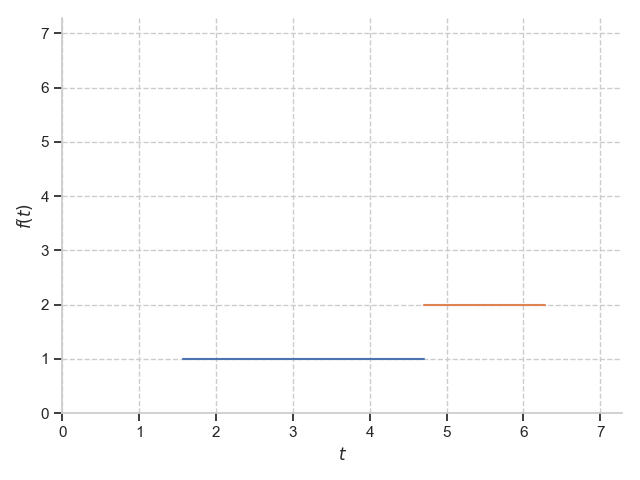
\includegraphics[scale=0.8]{f(t)sqwave.png}
    \captionsetup{skip=0pt}
    \caption{График $f(t)$ квадратной волны}
    \label{Рис:1}
\end{figure}


\noindent Теперь найдем коэффициенты $a_n,\,a_0,\,b_n,\,c_n$ и $\omega_n$ чтобы рассмотреть
частичные суммы рядов Фурье $F_N(t)$ и $G_N(t)$ следующего вида:
$$F_N(t)=\frac{a_0}{2}+\sum_{n=1}^{N}(a_n\cos{(\omega_n t)}+b_n\sin{(\omega_n t)})\,\,\,\,\,\,\,\,\,\,\,\,\,\,\,
G_N(t)=\sum_{n=-N}^{N}c_n e^{i \omega_n t}\,\,\,\,\,\,\,\,\,\,\,\,\,\,\,\omega_n=\frac{2\pi n}{T}$$


\noindent Формулы $a_n,\,b_n,\,c_n$ в общем виде для квадратной волны будут выглядеть следующим образом:
\begin{align*}
    & a_n=\dfrac{2}{T}\int\limits_{h}^{h+T}f(t)\cos{(\omega_n t)}\,dt=\dfrac{2}{1.5\pi}\left(\,\int\limits_{0.5\pi}^{1.5\pi}\cos{\left(\dfrac{2\pi n}{1.5\pi}t\right)}\,dt + \int\limits_{1.5\pi}^{2\pi}2\cos{\left(\dfrac{2\pi n}{1.5\pi}t\right)}\,dt\right)=\dfrac{4}{3\pi}\left(\,\int\limits_{0.5\pi}^{1.5\pi}\cos{\left(\dfrac{4}{3}nt\right)}\,dt+\right.\\
    & \left.=+2\int\limits_{1.5\pi}^{2\pi}\cos{\left(\dfrac{4}{3}nt\right)}\,dt\right)=
    \begin{bmatrix}
        x=\frc{4}{3}nt\\
        t=\frc{3}{4n}x\\
        dt=\frc{3}{4n}\,dx
    \end{bmatrix}
    =\dfrac{4}{3\pi}\cdot\dfrac{3}{4n}\left(\,\int\limits_{x_1=\frac{4}{3}n\cdot0.5\pi=\frac{2}{3}\pi n}^{x_2=\frac{4}{3}n\cdot1.5\pi=2\pi n}\cos{(x)}\,dx+2\int\limits_{x_3=\frac{4}{3}n\cdot1.5\pi=2\pi n}^{x_4=\frac{4}{3}n\cdot 2\pi=\frac{8}{3}\pi n}\cos{(x)}\,dx\right)=\\
    & =\dfrac{1}{\pi n}\left(\sin{(x)}\bigg|_{\frac{2}{3}\pi n}^{2\pi n}+2\sin{(x)}\bigg|_{2\pi n}^{\frac{8}{3}\pi n}\right)=\dfrac{1}{\pi n}\left(-\sin{(2\pi n)}-\sin{\left(\dfrac{2}{3}\pi n\right)}+2\sin{\left(\dfrac{8}{3}\pi n\right)}\right)\\
    & b_n=\dfrac{2}{T}\int\limits_{h}^{h+T}f(t)\sin{(\omega_n t)}\,dt=\dfrac{2}{1.5\pi}\left(\,\int\limits_{0.5\pi}^{1.5\pi}\sin{\left(\dfrac{2\pi n}{1.5\pi}t\right)}\,dt + \int\limits_{1.5\pi}^{2\pi}2\sin{\left(\dfrac{2\pi n}{1.5\pi}t\right)}\,dt\right)=\dfrac{4}{3\pi}\left(\,\int\limits_{0.5\pi}^{1.5\pi}\sin{\left(\dfrac{4}{3}nt\right)}\,dt+\right.\\
    & \left.+2\int\limits_{1.5\pi}^{2\pi}\sin{\left(\dfrac{4}{3}nt\right)}\,dt\right)=
    \begin{bmatrix}
        x=\frc{4}{3}nt\\
        t=\frc{3}{4n}x\\
        dt=\frc{3}{4n}\,dx
    \end{bmatrix}
    =\dfrac{4}{3\pi}\cdot\dfrac{3}{4n}\left(\,\int\limits_{x_1=\frac{4}{3}n\cdot0.5\pi=\frac{2}{3}\pi n}^{x_2=\frac{4}{3}n\cdot1.5\pi=2\pi n}\sin{(x)}\,dx+2\int\limits_{x_3=\frac{4}{3}n\cdot1.5\pi=2\pi n}^{x_4=\frac{4}{3}n\cdot 2\pi=\frac{8}{3}\pi n}\sin{(x)}\,dx\right)=\\
    & = -\dfrac{1}{\pi n}\left(\cos{(x)}\bigg|_{\frac{2}{3}\pi n}^{2\pi n}+2\cos{(x)}\bigg|_{2\pi n}^{\frac{8}{3}\pi n}\right)=-\dfrac{1}{\pi n}\left(-\cos{(2\pi n)}-\cos{\left(\dfrac{2}{3}\pi n\right)}+2\cos{\left(\dfrac{8}{3}\pi n\right)}\right)\\
    & c_n=\dfrac{1}{T}\int\limits_{h}^{h+T}f(t)e^{-i \omega_n t}\,dt=\dfrac{1}{1.5\pi}\left(\,\int\limits_{0.5\pi}^{1.5\pi} e^{-i \frac{2\pi n}{1.5\pi}t}\,dt+\int\limits_{1.5\pi}^{2\pi}2e^{-i \frac{2\pi n}{1.5\pi}t}\,dt\right)=\dfrac{2}{3\pi}\left(\,\int\limits_{0.5\pi}^{1.5\pi}e^{-i\frac{4}{3}nt}\,dt + 2\int\limits_{1.5\pi}^{2\pi}e^{-i\frac{4}{3}nt}\,dt\right)=\\
    & =
    \begin{bmatrix}
        x=-\dfrac{4}{3}int, &t=-\dfrac{3}{4ni}x=\dfrac{3i}{4n}x, &dt=\dfrac{3i}{4n}\,dx
    \end{bmatrix}
    =\dfrac{2}{3\pi}\cdot\dfrac{3i}{4n}\left(\,\int\limits_{x_1=-\frac{4}{3}in\cdot0.5\pi=-\frac{2}{3}\pi i n}^{x_2=-\frac{4}{3}in\cdot1.5\pi=-2\pi i n}e^{x}\,dx + 2\int\limits_{x_3=x_1=-2\pi i n}^{x_4=-\frac{4}{3}i n \cdot 2\pi=-\frac{8}{3}\pi i n}e^{x}\,dx\right)=\\
    & =\dfrac{i}{2\pi n}\left(e^{x}\bigg|_{-\frac{2}{3}\pi i n}^{-2\pi i n}+2e^{x}\bigg|_{-2\pi i n}^{-\frac{8}{3}\pi i n}\right)=\dfrac{i}{2\pi n}(-e^{-2\pi i n}-e^{-\frac{2}{3}\pi i n}+2e^{-\frac{8}{3}\pi i n})\\
    & a_0=\dfrac{2}{T}\int\limits_{h}^{h+T}f(t)\,dt=\dfrac{2}{1.5\pi}\left(\,\int\limits_{0.5\pi}^{1.5\pi}1\,dt+\int\limits_{1.5\pi}^{2\pi}2\,dt\right)=\dfrac{4}{3\pi}\left(t\bigg|_{0.5\pi}^{1.5\pi}+2t\bigg|_{1.5\pi}^{2\pi}\right)=\dfrac{4}{3\pi}(1.5\pi-0.5\pi+2(2\pi-1.5\pi))=\dfrac{8}{3}
\end{align*}


\noindent Теперь составим $F_N(t)$ и $G_N(t)$:
\begin{align*}
    & F_N(t)=\dfrac{4}{3}+\sum_{n=1}^{N}\dfrac{1}{\pi n}\left(\left(-\sin{(2\pi n)}-\sin{\left(\dfrac{2}{3}\pi n\right)}+2\sin{\left(\dfrac{8}{3}\pi n\right)}\right)\cos{\left(\dfrac{4}{3}nt\right)}+\right.\\
    & \left.+\left(\cos{(2\pi n)}+\cos{\left(\dfrac{2}{3}\pi n\right)}-2\cos{\left(\dfrac{8}{3}\pi n\right)}\right)\sin{\left(\dfrac{4}{3}nt\right)}\right)\\
    & G_N(t)=\sum_{n=-N}^{N}\dfrac{i}{2\pi n}(-e^{-2\pi i n}-e^{-\frac{2}{3}\pi i n}+2e^{-\frac{8}{3}\pi i n})e^{\frac{4i}{3}nt}
\end{align*}


\noindent Теперь вычислим значения коэффициентов при $n=0,1,2$. Значение $a_0=\frc{8}{3}$ было вычислено выше. Получим:
\begin{align*}
    & a_1=\dfrac{1}{\pi}\left(-\sin{(2\pi)}-\sin{\left(\dfrac{2}{3}\pi\right)}+2\sin{\left(\dfrac{8}{3}\pi\right)}\right)=\dfrac{\sqrt{3}}{2\pi}\approx 0.28\\
    & a_2=\dfrac{1}{2\pi}\left(-\sin{(4\pi)}-\sin{\left(\dfrac{4}{3}\pi\right)}+2\sin{\left(\dfrac{16}{3}\pi\right)}\right)=-\dfrac{\sqrt{3}}{4\pi}\approx -0.14\\
    & b_0=0, \text{ так как при } n=0\Rightarrow \omega_n=\dfrac{2\pi\cdot 0}{1.5\pi}=0\Rightarrow \dfrac{2}{T}\int\limits_{h}^{h+T}f(t)\sin{(0)}\,dt=0\\
    & b_1=\dfrac{1}{\pi}\left(\cos{(2\pi)}+\cos{\left(\dfrac{2}{3}\pi\right)}-2\cos{\left(\dfrac{8}{3}\pi\right)}\right)=\dfrac{3}{2\pi}\approx 0.48\\
    & b_2=\dfrac{1}{2\pi}\left(\cos{(4\pi)}+\cos{\left(\dfrac{4}{3}\pi\right)}-2\cos{\left(\dfrac{16}{3}\pi\right)}\right)=\dfrac{3}{4\pi}\approx 0.24\\
    & c_0=\dfrac{a_0}{2}=\dfrac{\frc{8}{3}}{2}=\dfrac{4}{3}\approx 1.33, \text{ так как при } n=0\Rightarrow \omega_n=0\Rightarrow\dfrac{1}{T}\int\limits_{h}^{h+T}f(t)e^{0}\,dt=\dfrac{1}{T}\int\limits_{h}^{h+T}f(t)\,dt,\\
    & \text{что отличается от } a_0 \text{ коэффициентом } \dfrac{1}{T} \text{ вместо } \dfrac{2}{T}\Rightarrow c_0=\dfrac{a_0}{2}\\
    & c_1=\dfrac{i}{2\pi}(-e^{-2\pi i}-e^{-\frac{2}{3}\pi i}+2e^{-\frac{8}{3}\pi i})\approx 0.14-0.24i\\
    & c_2=\dfrac{i}{4\pi}(-e^{-4\pi i}-e^{-\frac{4}{3}\pi i}+2e^{-\frac{16}{3}\pi i})\approx -0.07-0.12i
\end{align*}


\newpage
\noindent Для вычисления коэффициентов ряда Фурье при произвольно заданном значении N я написал следующий код:
\begin{lstlisting}
import sympy as sp

t = sp.Symbol('t')

def calc_coeff(complex: bool, gap_len):
    if complex:
        return 1 / gap_len
    return 2 / gap_len

def calc_omega_n(n, gap_len):
    return 2 * sp.pi * n / gap_len

def calc_a_n(n, start, end, gap_len, f):
    integrand = f(t)
    if n != 0:
        omega_n = calc_omega_n(n, gap_len)
        integrand *= sp.cos(omega_n * t)
        
    result = sp.integrate(integrand, (t, start, end))

    coeff = calc_coeff(False, gap_len)
    return coeff * result

def calc_b_n(n, start, end, gap_len, f):
    if (n == 0):
        return 0

    omega_n = calc_omega_n(n, gap_len)
    integrand = f(t) * sp.sin(omega_n * t)
        
    result = sp.integrate(integrand, (t, start, end))

    coeff = calc_coeff(False, gap_len)
    return coeff * result

def calc_c_n(n, start, end, gap_len, f):
    omega_n = calc_omega_n(n, gap_len)
    integrand = f(t) * sp.exp(-1j * omega_n * t)

    result = sp.integrate(integrand, (t, start, end))

    coeff = calc_coeff(True, gap_len)
    return coeff * result
\end{lstlisting}


\noindent Пример использования кода:
\begin{lstlisting}
funcs = [square_wave_a, square_wave_b]
def find_a_b_c(N):
    a_N = sum(calc_a_n(N, gap[0], gap[1], gap_len, funcs[i])
              for i, gap in enumerate(gaps))
    b_N = sum(calc_b_n(N, gap[0], gap[1], gap_len, funcs[i])
              for i, gap in enumerate(gaps))
    c_N = sum(calc_c_n(N, gap[0], gap[1], gap_len, funcs[i]) 
              for i, gap in enumerate(gaps))

    print(f'a_{N}={a_N}\n')
    print(f'b_{N}={b_N}\n')
    print(f'c_{N}={c_N}\n')
find_a_b_c(N)
\end{lstlisting}


\noindent Найдем с помощью него коэффицинты при N=3. Для наглядности были добавлены вычисления для N=0, 1, 2.
Результат выполнения кода:
\begin{lstlisting}
a_0=2.66666666666667   b_0=0                 c_0=1.33333333333333
a_1=0.275664447710896  b_1=0.477464829275686 c_1=0.137832223855448 - 0.238732414637843*I
a_2=-0.137832223855448 b_2=0.238732414637843 c_2=-0.0689161119277239 - 0.119366207318922*I
a_3=0                  b_3=0                 c_3=-0.e-261 + 0.e-255*I
\end{lstlisting}


\noindent Теперь построим графики $F_N(t)$ и $G_N(t)$ при различных значениях N. Ряд Фурье
построен зеленым цветом поверх заданной функции $f(t)$
\newpage
\noindent Для построения графика $F_N(t)$ при разных значениях функции на разных интервалах я написал следующий код:
\begin{lstlisting}
def calc_F_N_generic(N, gaps: list, functions: list):
    if (len(gaps) != len(functions) 
        or len(gaps) <= 0 
        or len(functions) <= 0):
        return None

    gap_len = gaps[-1][1] - gaps[0][0]

    a_0 = sum(calc_a_n(0, gap[0], gap[1], gap_len, functions[i]) 
              for i, gap in enumerate(gaps))

    F_N = a_0 / 2
    for n in range(1, N + 1):
        a_n = sum(calc_a_n(n, gap[0], gap[1], gap_len, functions[i]) 
                  for i, gap in enumerate(gaps))
        b_n = sum(calc_b_n(n, gap[0], gap[1], gap_len, functions[i]) 
                  for i, gap in enumerate(gaps))

        omega_n = calc_omega_n(n, gap_len)
        F_N += a_n * sp.cos(omega_n * t) + b_n * sp.sin(omega_n * t)

    return F_N
\end{lstlisting}


\noindent Для $G_N(t)$:
\begin{lstlisting}
def calc_G_N_generic(N, gaps: list, functions: list):
    if (len(gaps) != len(functions) 
        or len(gaps) <= 0 
        or len(functions) <= 0):
        return None

    G_N = 0
    gap_len = gaps[-1][1] - gaps[0][0]
    for n in range(-N, N + 1):
        c_n = sum(calc_c_n(n, gap[0], gap[1], gap_len, functions[i]) 
                  for i, gap in enumerate(gaps))
        
        omega_n = calc_omega_n(n, gap_len)
        G_N += c_n * sp.exp(1j * omega_n * t)

    return G_N
\end{lstlisting}


\noindent Пример использования кода:
\begin{lstlisting}
def build_F_N__f_t(N):
    F_N = calc_F_N_generic(N, gaps, funcs)
    sp.plot((f_t_1, (t, gaps[0][0], gaps[0][1])), 
            (f_t_2, (t, gaps[1][0], gaps[1][1])), 
            (F_N, (t, gaps[0][0], gaps[-1][1])),
            axis_center=(0, 0), xlim=(0, gap_end_val + 1), 
            ylim=(0, gap_end_val + 1), xlabel=r'$t$', 
            ylabel=r'$f(t)$')

def build_G_N__f_t(N):
    G_N = calc_G_N_generic(N, gaps, funcs)
    sp.plot((f_t_1, (t, gaps[0][0], gaps[0][1])), 
            (f_t_2, (t, gaps[1][0], gaps[1][1])), 
            (G_N, (t, gaps[0][0], gaps[-1][1])),
            axis_center=(0, 0), xlim=(0, gap_end_val + 1), 
            ylim=(0, gap_end_val + 1), xlabel=r'$t$', 
            ylabel=r'$f(t)$')
build_F_N__f_t(N_1)
build_F_N__f_t(N_2)
build_F_N__f_t(N_3)
build_F_N__f_t(N_4)
build_F_N__f_t(N_5)
build_G_N__f_t(N_1)
build_G_N__f_t(N_2)
build_G_N__f_t(N_3)
build_G_N__f_t(N_4)
build_G_N__f_t(N_5)
\end{lstlisting}


\noindent Далее приведены графики $F_N(t)$ и $G_N(t)$ при N=10, 20, 30, 40, 50


\newpage
\vspace*{10mm}
\begin{figure}[!htb]
    \centering
    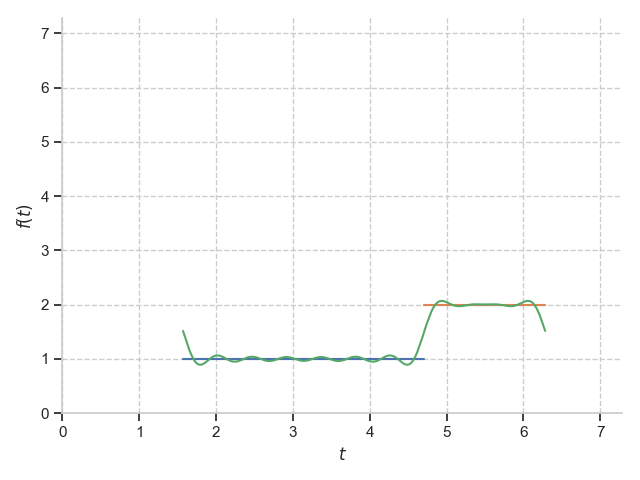
\includegraphics[scale=0.8]{fur_sqwave_n=10.png}
    \captionsetup{skip=0pt}
    \caption{График $F_N(t)$ квадратной волны при N=10}
    \label{Рис:2}
\end{figure}
\begin{figure}[!htb]
    \centering
    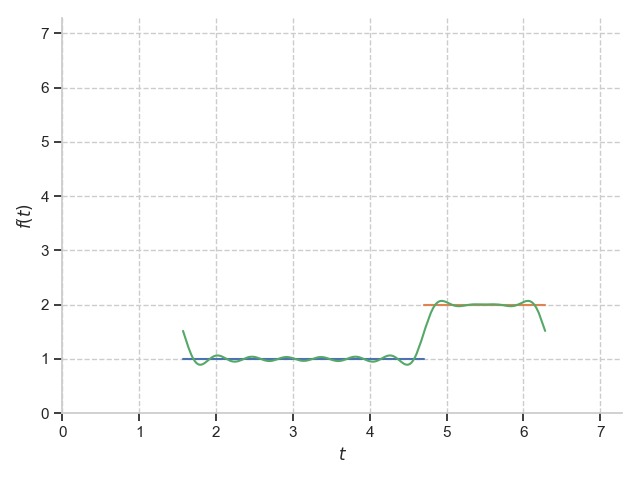
\includegraphics[scale=0.8]{cfur_sqwave_n=10.png}
    \captionsetup{skip=0pt}
    \caption{График $G_N(t)$ квадратной волны при N=10}
    \label{Рис:3}
\end{figure}
\newpage
\vspace*{10mm}
\begin{figure}[!htb]
    \centering
    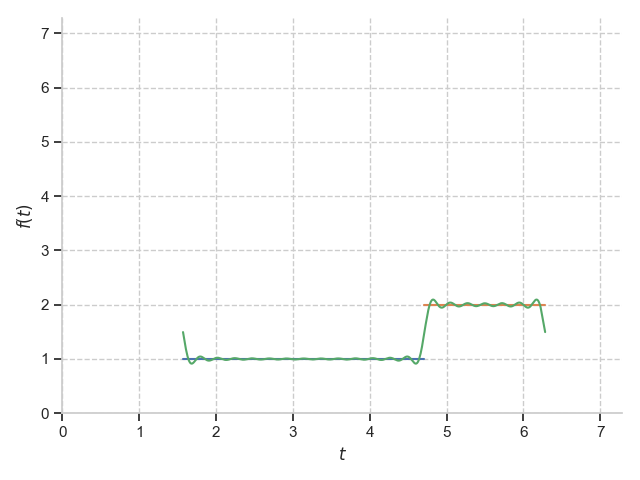
\includegraphics[scale=0.8]{fur_sqwave_n=20.png}
    \captionsetup{skip=0pt}
    \caption{График $F_N(t)$ квадратной волны при N=20}
    \label{Рис:4}
\end{figure}
\begin{figure}[!htb]
    \centering
    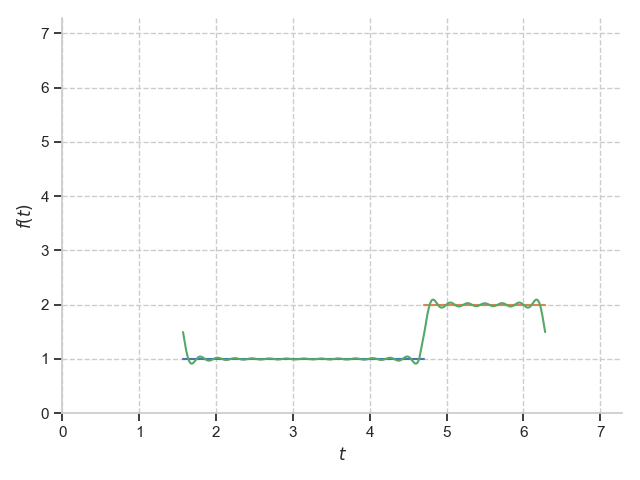
\includegraphics[scale=0.8]{cfur_sqwave_n=20.png}
    \captionsetup{skip=0pt}
    \caption{График $G_N(t)$ квадратной волны при N=20}
    \label{Рис:5}
\end{figure}
\newpage
\vspace*{10mm}
\begin{figure}[!htb]
    \centering
    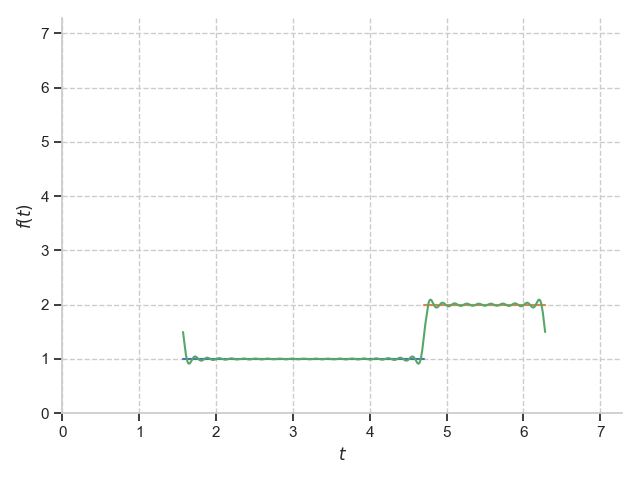
\includegraphics[scale=0.8]{fur_sqwave_n=30.png}
    \captionsetup{skip=0pt}
    \caption{График $F_N(t)$ квадратной волны при N=30}
    \label{Рис:6}
\end{figure}
\begin{figure}[!htb]
    \centering
    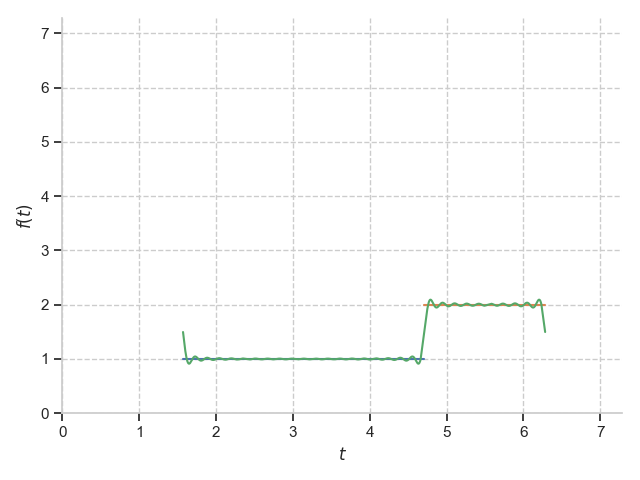
\includegraphics[scale=0.8]{cfur_sqwave_n=30.png}
    \captionsetup{skip=0pt}
    \caption{График $G_N(t)$ квадратной волны при N=30}
    \label{Рис:7}
\end{figure}
\newpage
\vspace*{10mm}
\begin{figure}[!htb]
    \centering
    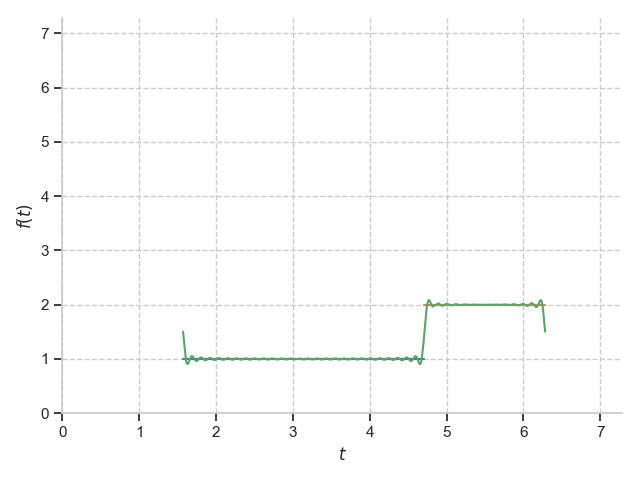
\includegraphics[scale=0.8]{fur_sqwave_n=40.png}
    \captionsetup{skip=0pt}
    \caption{График $F_N(t)$ квадратной волны при N=40}
    \label{Рис:8}
\end{figure}
\begin{figure}[!htb]
    \centering
    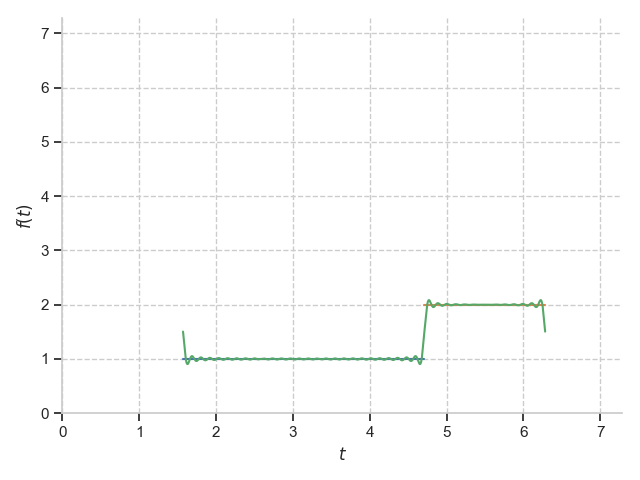
\includegraphics[scale=0.8]{cfur_sqwave_n=40.png}
    \captionsetup{skip=0pt}
    \caption{График $G_N(t)$ квадратной волны при N=40}
    \label{Рис:9}
\end{figure}
\newpage
\begin{figure}[!htb]
    \centering
    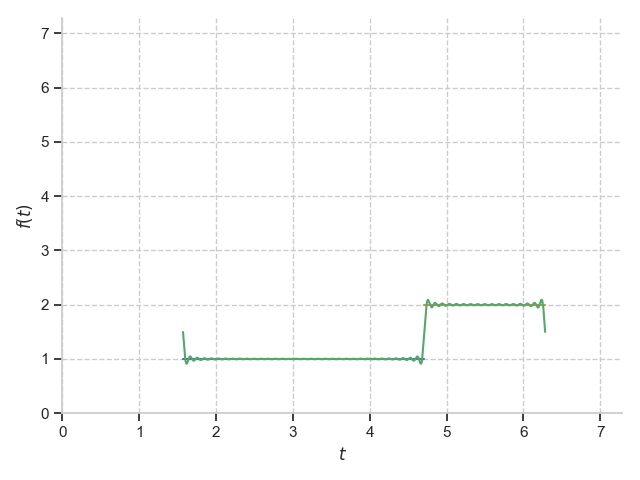
\includegraphics[scale=0.8]{fur_sqwave_n=50.png}
    \captionsetup{skip=0pt}
    \caption{График $F_N(t)$ квадратной волны при N=50}
    \label{Рис:10}
\end{figure}
\begin{figure}[!htb]
    \centering
    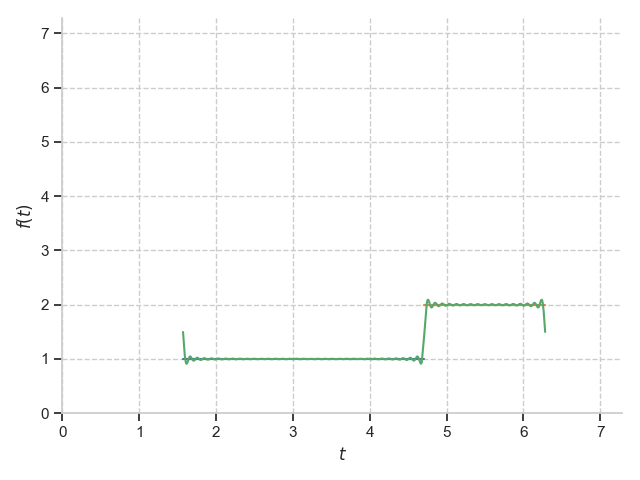
\includegraphics[scale=0.8]{cfur_sqwave_n=50.png}
    \captionsetup{skip=0pt}
    \caption{График $G_N(t)$ квадратной волны при N=50}
    \label{Рис:11}
\end{figure}


\noindent Как можно заметить, чем больше значение N, тем точнее
ряд Фурье повторяет изначально заданную функцию $f(t)$. Уже при N=50
функцию $f(t)$ почти не видно за функцией $F_N(t)$ или $G_N(t)$. За простоту написания
$G_N(t)$ мы платим сложностью алгоритма -- в $G_N(t)$ два раза больше итераций, чем в $F_N(t)$.
Так как обе функции описывают одну и ту же $f(t)$, то результат на графиках будет одинаковым


\newpage
\noindent Равенство Парсеваля выглядит следующим образом:
\begin{align*}
    & \sum_{n=-\infty}^{\infty}|c_n|^2=\dfrac{1}{T}\int\limits_{a}^{b}|f(t)|^2\,dt,
\end{align*}
\noindent где $|c_n|^2=(\text{Re}\,c_n)^2+(\text{Im}\,c_n)^2,\,\,|f(t)|^2=f^{*}(t)f(t)$

\noindent Для проверки равенства Парсеваля я написал следующий код:
\begin{lstlisting}
def calc_parseval_coeffs_generic(N, gaps: list, functions: list):
    if (len(gaps) != len(functions) 
        or len(gaps) <= 0 
        or len(functions) <= 0):
        return None
        
    coeffs = 0
    gap_len = gaps[-1][1] - gaps[0][0]
    for n in range(-N, N + 1):
        c_n = sum(calc_c_n(n, gap[0], gap[1], gap_len, functions[i]) 
                for i, gap in enumerate(gaps))
            
        coeffs += sp.re(c_n) ** 2 + sp.im(c_n) ** 2

    return coeffs

def calc_parseval_square_func_generic(gaps: list, functions: list):
    result = 0
    for i in range(len(gaps)):
        integrand = functions[i] * sp.conjugate(functions[i])
        result += sp.integrate(integrand, (t, gaps[i][0], gaps[i][1]))
        
    gap_len = gaps[-1][1] - gaps[0][0]
    return (1 / gap_len) * result
\end{lstlisting}


\noindent Пример использования кода:
\begin{lstlisting}
f_t_1 = square_wave_a(t)
f_t_2 = square_wave_b(t)
funcs = [square_wave_a, square_wave_b]
funcs_t = [f_t_1, f_t_2]
def find_parseval(N):
    coeffs_sum = calc_parseval_coeffs_generic(N, gaps, funcs)
    sqf_res = calc_parseval_square_func_generic(gaps, funcs_t)

    print(f'coeffs_sum={coeffs_sum.evalf()}')
    print(f'sqf_res={sqf_res.evalf()}')
find_parseval(N)
\end{lstlisting}


\noindent Результат проверки для N=10:
\begin{lstlisting}
coeffs_sum=1.99032933097543    sqf_res=2.00000000000000
\end{lstlisting}


\noindent Результат проверки для N=25:
\begin{lstlisting}
coeffs_sum=1.99602510318456    sqf_res=2.00000000000000
\end{lstlisting}


\noindent Результат проверки для N=50:
\begin{lstlisting}
coeffs_sum=1.99801369165273    sqf_res=2.00000000000000
\end{lstlisting}


\noindent Результат проверки для N=100:
\begin{lstlisting}
coeffs_sum=1.99899180407561    sqf_res=2.00000000000000
\end{lstlisting}


\noindent Как видим, сумма коэффициентов c увеличением N приближается к
вычисленному значению интеграла квадрата функции $f(t)$. Равенство Парсеваля
не выполняется в чистом виде, так как коэффициентов бесконечно много, а мы взяли
лишь малую их часть. То есть мы наблюдаем стремление к равенству Парсеваля, а 
выполнение равенства Парсеваля было бы при равенстве нулю всех коэффициентов кроме одного


\newpage
\subsection{Чётная периодическая функция}
Зададим следующую чётную периодическую функцию:
$$f(t)=\cos(t)$$


\noindent Для построения графика $f(t)$ будем использовать следующий код:
\begin{lstlisting}[belowskip=-3mm]
f_t = even_periodic_func(t)

def build_f_t():
    sp.plot((f_t, (t, gaps[0][0], gaps[-1][1])), 
            axis_center=(0, 0), xlim=(0, gap_end_val + 1), 
            ylim=(-1.5, 1.5), xlabel=r'$t$', ylabel=r'$f(t)$')
\end{lstlisting}
\begin{figure}[!htb]
    \centering
    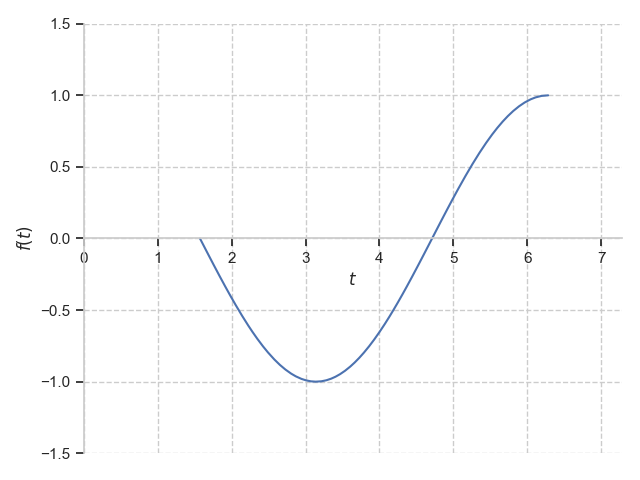
\includegraphics[scale=0.8]{even_f(t).png}
    \captionsetup{skip=0pt}
    \caption{График $f(t)$ чётной периодической функции}
    \label{Рис:12}
\end{figure}


\noindent Формулы для вычисления коэффициентов $a_n,\,a_0,\,b_n,\,c_n$ будут иметь вид:
\begin{align*}
    & a_n=\dfrac{4}{3\pi}\int\limits_{0.5\pi}^{2\pi}\cos{(t)\cdot \cos{\left(\dfrac{4}{3}nt\right)}}\,dt=\dfrac{2\left((4n-3)\left(\cos{\left(\dfrac{2{\pi}n}{3}\right)}-\sin{\left(\dfrac{8{\pi}n}{3}\right)}\right)-(4n+3)\left(\cos{\left(\dfrac{2{\pi}n}{3}\right)}+\sin{\left(\dfrac{8{\pi}n}{3}\right)}\right)\right)}{{\pi}\left(9-16n^2\right)}\\
    & b_n=\dfrac{4}{3\pi}\int\limits_{0.5\pi}^{2\pi}\cos{(t)}\cdot\sin{\left(\dfrac{4}{3}nt\right)}\,dt=\dfrac{2\left((4n-3)\left(\cos{\left(\dfrac{8{\pi}n}{3}\right)}+\sin{\left(\dfrac{2{\pi}n}{3}\right)}\right)+(4n+3)\left(\cos\left(\dfrac{8{\pi}n}{3}\right)-\sin{\left(\dfrac{2{\pi}n}{3}\right)}\right)\right)}{{\pi}\left(9-16n^2\right)}\\
    & c_n=\dfrac{2}{3\pi}\int\limits_{0.5\pi}^{2\pi}\cos{(t)}\cdot e^{-\frac{4i}{3}nt}\,dt=\dfrac{2}{\pi(16n^2-9)}\left(4n\left(\sin{\left(\dfrac{8\pi n}{3}\right)}+i\cos{\left(\dfrac{8\pi n}{3}\right)}\right)+3\left(\cos{\left(\dfrac{2\pi n}{3}\right)}-i\sin{\left(\dfrac{2\pi n}{3}\right)}\right)\right)\\
    & a_0=\dfrac{4}{3\pi}\int\limits_{0.5\pi}^{2\pi}\cos{(t)}\,dt=\dfrac{4}{3\pi}\sin{(t)}\bigg|_{0.5\pi}^{2\pi}=-\dfrac{4}{3\pi}
\end{align*}


\noindent Теперь составим $F_N(t)$ и $G_N(t)$:
\begin{align*}
    & F_N(t)=-\dfrac{2}{3\pi}+\sum_{n=1}^{N}\dfrac{2\left((4n-3)\left(\cos{\left(\dfrac{2{\pi}n}{3}\right)}-\sin{\left(\dfrac{8{\pi}n}{3}\right)}\right)-(4n+3)\left(\cos{\left(\dfrac{2{\pi}n}{3}\right)}+\sin{\left(\dfrac{8{\pi}n}{3}\right)}\right)\right)}{{\pi}\left(9-16n^2\right)}\cos{\left(\dfrac{4}{3}nt\right)}+\\
    & +\dfrac{2\left((4n-3)\left(\cos{\left(\dfrac{8{\pi}n}{3}\right)}+\sin{\left(\dfrac{2{\pi}n}{3}\right)}\right)+(4n+3)\left(\cos\left(\dfrac{8{\pi}n}{3}\right)-\sin{\left(\dfrac{2{\pi}n}{3}\right)}\right)\right)}{{\pi}\left(9-16n^2\right)}\sin{\left(\dfrac{4}{3}nt\right)}\\
    & G_N(t)=\sum_{n=-N}^{N}\dfrac{2e^{\frac{4i}{3}nt}}{\pi(16n^2-9)}\left(4n\left(\sin{\left(\dfrac{8\pi n}{3}\right)}+i\cos{\left(\dfrac{8\pi n}{3}\right)}\right)+3\left(\cos{\left(\dfrac{2\pi n}{3}\right)}-i\sin{\left(\dfrac{2\pi n}{3}\right)}\right)\right)
\end{align*}


\noindent С помощью приведенного ранее кода найдем значения коэффициентов при N=3:
\begin{lstlisting}
a_3=0.0282942121052258
b_3=-0.113176848420903
c_3=0.0141471060526129 + 0.0565884242104517*I
\end{lstlisting}


\noindent Построим графики $F_N(t)$ и $G_N(t)$. Для случая с одной функцией и одним интервалом я написал
упрощенную версию кода. Для $F_N(t)$ имеем:
\begin{lstlisting}
def calc_F_N(N, start, end, f):
    gap_len = end - start

    a_0 = calc_a_n(0, start, end, gap_len, f)

    F_N = a_0 / 2
    for n in range(1, N + 1):
        a_n = calc_a_n(n, start, end, gap_len, f)
        b_n = calc_b_n(n, start, end, gap_len, f)

        omega_n = calc_omega_n(n, gap_len)
        F_N += a_n * sp.cos(omega_n * t) + b_n * sp.sin(omega_n * t)

    return F_N
\end{lstlisting}


\noindent Для $G_N$:
\begin{lstlisting}
def calc_G_N(N, start, end, f):
    G_N = 0
    gap_len = end - start
    for n in range(-N, N + 1):
        c_n = calc_c_n(n, start, end, gap_len, f)

        omega_n = calc_omega_n(n, gap_len)
        G_N += c_n * sp.exp(1j * omega_n * t)

    return G_N
\end{lstlisting}


\noindent Пример использования кода:
\begin{lstlisting}
def build_F_N__f_t(N):
    F_N = calc_F_N(N, gaps[0][0], gaps[-1][1], even_periodic_func)
    sp.plot((f_t, (t, gaps[0][0], gaps[-1][1])), 
            (F_N, (t, gaps[0][0], gaps[-1][1])), 
            axis_center=(0, 0), xlim=(0, gap_end_val + 1), 
            ylim=(-1.5, 1.5), xlabel=r'$t$', ylabel=r'$f(t)$')

def build_G_N__f_t(N):
    G_N = calc_G_N(N, gaps[0][0], gaps[-1][1], even_periodic_func)
    sp.plot((f_t, (t, gaps[0][0], gaps[-1][1])), 
            (G_N, (t, gaps[0][0], gaps[-1][1])), 
            axis_center=(0, 0), xlim=(0, gap_end_val + 1), 
            ylim=(-1.5, 1.5), xlabel=r'$t$', ylabel=r'$f(t)$')
build_F_N__f_t(N_1)
build_F_N__f_t(N_2)
build_F_N__f_t(N_3)
build_F_N__f_t(N_4)
build_F_N__f_t(N_5)
build_G_N__f_t(N_1)
build_G_N__f_t(N_2)
build_G_N__f_t(N_3)
build_G_N__f_t(N_4)
build_G_N__f_t(N_5)
\end{lstlisting}


\noindent Далее приведены графики $F_N(t)$ и $G_N(t)$ оранжевым цветом поверх функции $f(t)$
\newpage
\vspace*{10mm}
\begin{figure}[!htb]
    \centering
    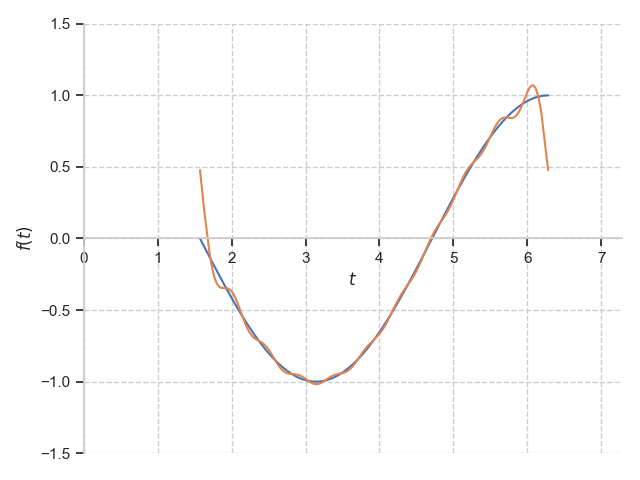
\includegraphics[scale=0.8]{fur_cos_n=10.png}
    \captionsetup{skip=0pt}
    \caption{График $F_N(t)$ чётной периодической функции при N=10}
    \label{Рис:13}
\end{figure}
\begin{figure}[!htb]
    \centering
    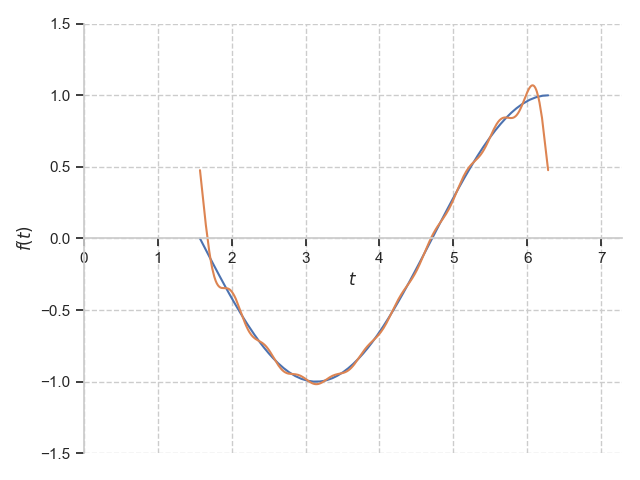
\includegraphics[scale=0.8]{cfur_cos_n=10.png}
    \captionsetup{skip=0pt}
    \caption{График $G_N(t)$ чётной периодической функции при N=10}
    \label{Рис:14}
\end{figure}
\newpage
\vspace*{10mm}
\begin{figure}[!htb]
    \centering
    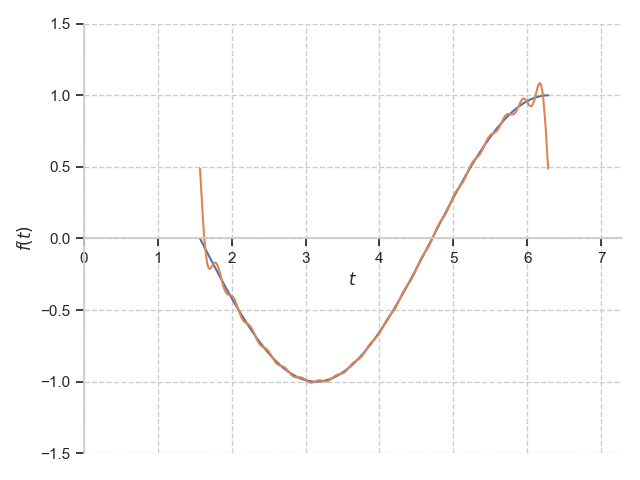
\includegraphics[scale=0.8]{fur_cos_n=20.png}
    \captionsetup{skip=0pt}
    \caption{График $F_N(t)$ чётной периодической функции при N=20}
    \label{Рис:15}
\end{figure}
\begin{figure}[!htb]
    \centering
    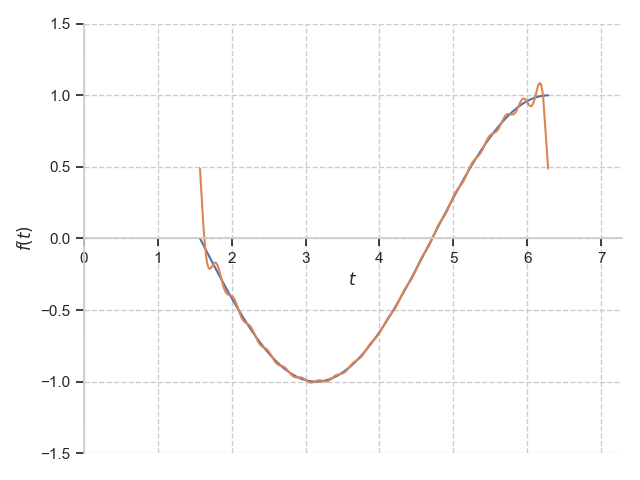
\includegraphics[scale=0.8]{cfur_cos_n=20.png}
    \captionsetup{skip=0pt}
    \caption{График $G_N(t)$ чётной периодической функции при N=20}
    \label{Рис:16}
\end{figure}
\newpage
\vspace*{10mm}
\begin{figure}[!htb]
    \centering
    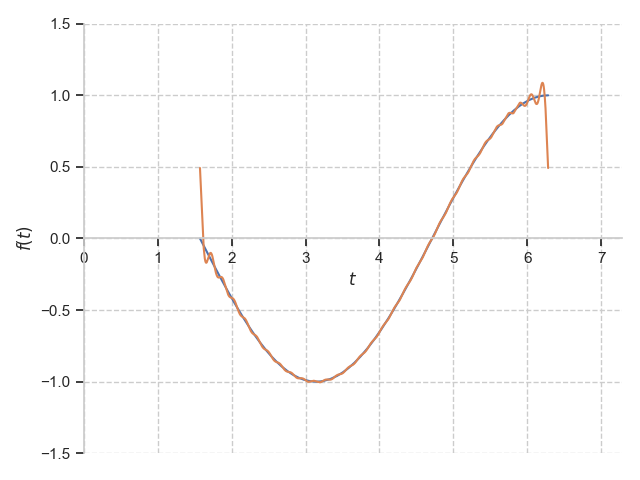
\includegraphics[scale=0.8]{fur_cos_n=30.png}
    \captionsetup{skip=0pt}
    \caption{График $F_N(t)$ чётной периодической функции при N=30}
    \label{Рис:17}
\end{figure}
\begin{figure}[!htb]
    \centering
    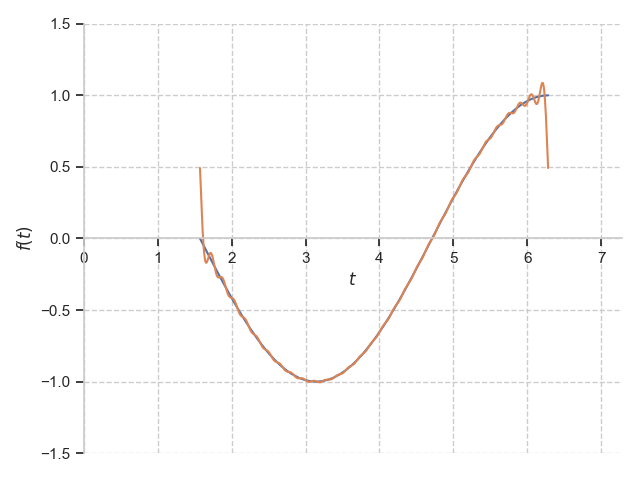
\includegraphics[scale=0.8]{cfur_cos_n=30.png}
    \captionsetup{skip=0pt}
    \caption{График $G_N(t)$ чётной периодической функции при N=30}
    \label{Рис:18}
\end{figure}
\newpage
\vspace*{10mm}
\begin{figure}[!htb]
    \centering
    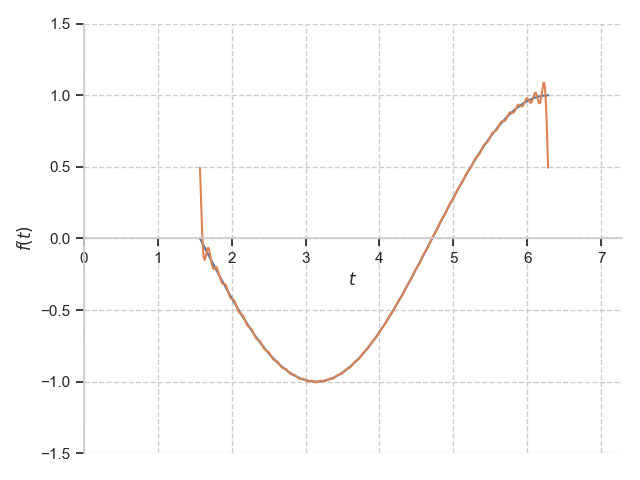
\includegraphics[scale=0.8]{fur_cos_n=40.png}
    \captionsetup{skip=0pt}
    \caption{График $F_N(t)$ чётной периодической функции при N=40}
    \label{Рис:19}
\end{figure}
\begin{figure}[!htb]
    \centering
    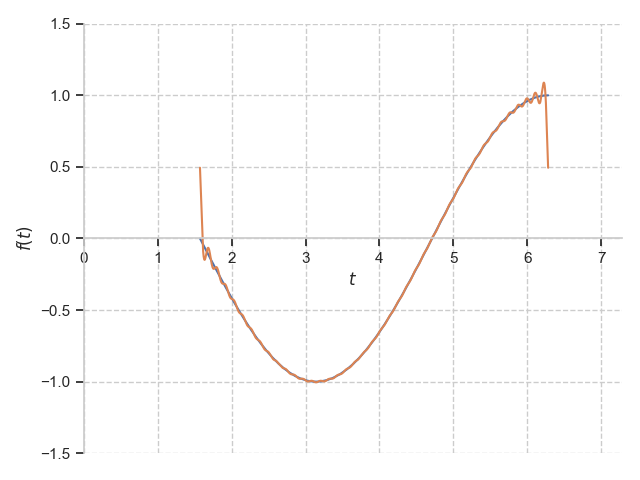
\includegraphics[scale=0.8]{cfur_cos_n=40.png}
    \captionsetup{skip=0pt}
    \caption{График $G_N(t)$ чётной периодической функции при N=40}
    \label{Рис:20}
\end{figure}
\newpage
\begin{figure}[!htb]
    \centering
    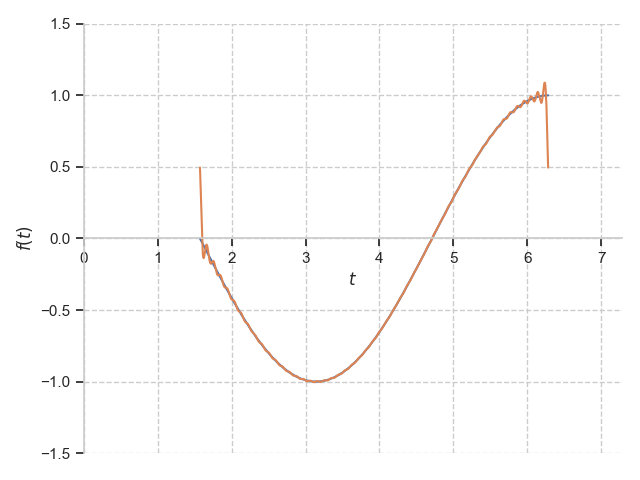
\includegraphics[scale=0.8]{fur_cos_n=50.png}
    \captionsetup{skip=0pt}
    \caption{График $F_N(t)$ чётной периодической функции при N=50}
    \label{Рис:21}
\end{figure}
\begin{figure}[!htb]
    \centering
    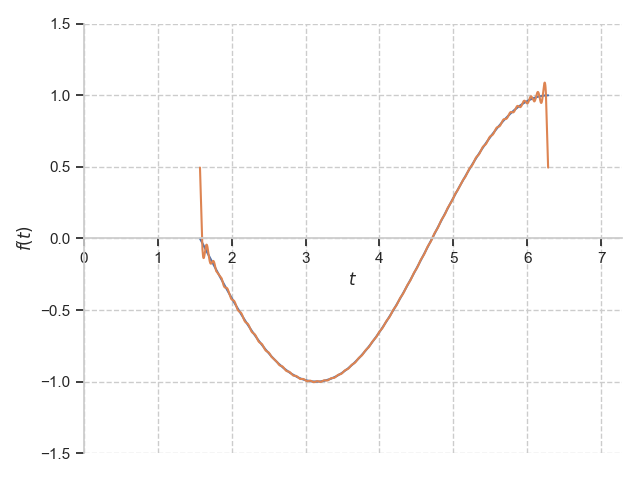
\includegraphics[scale=0.8]{cfur_cos_n=50.png}
    \captionsetup{skip=0pt}
    \caption{График $G_N(t)$ чётной периодической функции при N=50}
    \label{Рис:22}
\end{figure}


\noindent Исходя из полученных графиков можно сделать вывод, что приводить
и графики $F_N(t)$, и графики $G_N(t)$ в работе избыточно, так как они одинаковы, в чем
мы убедились еще тогда, когда строили квадратную волну. Поэтому далее в отчете я
буду приводить только графики $F_N(t)$. Тем не менее, графики $G_N(t)$ у меня построены
на каждую функцию в пяти экземплярах



\noindent Так как функция $f(t)$ чётная, то в частичных суммах ряда
Фурье преобладают косинусы, поэтому графики очень похожи. Если рассматривать функцию $f(t)$
с периодом $2\pi$, например на промежутке $[0.5\pi, 2.5\pi]$, то графики $F_N(t)$ и $G_N(t)$ будут
совпадать с графиком $f(t)$, так как все $b_n$ занулятся


\newpage
\noindent Для проверки равенства Парсеваля для одной функции на одном интервале я написал упрощенную версию кода:
\begin{lstlisting}
def calc_parseval_coeffs(N, start, end, f):
    coeffs = 0
    gap_len = end - start
    for n in range(-N, N + 1):
        c_n = calc_c_n(n, start, end, gap_len, f)

        coeffs += sp.re(c_n) ** 2 + sp.im(c_n) ** 2

    return coeffs
def calc_parseval_square_func(start, end, f):
    integrand = f * sp.conjugate(f)

    result = sp.integrate(integrand, (t, start, end))

    gap_len = end - start
    return (1 / gap_len) * result
\end{lstlisting}


\noindent Пример использования упрощенной версии кода:
\begin{lstlisting}
def find_parseval(N):
    coeffs_sum = calcs.calc_parseval_coeffs(N, gaps[0][0], gaps[-1][1], even_periodic_func)
    sqf_res = calcs.calc_parseval_square_func(gaps[0][0], gaps[-1][1], even_periodic_func(t))

    print(f'coeffs_sum={coeffs_sum.evalf()}')
    print(f'sqf_res={sqf_res.evalf()}')
find_parseval(N)
\end{lstlisting}


\noindent Результат выполнения кода для N=10
\begin{lstlisting}
coeffs_sum=0.495154186636485    sqf_res=0.500000000000000
\end{lstlisting}


\noindent Результат выполнения кода для N=25
\begin{lstlisting}
coeffs_sum=0.498011845838439    sqf_res=0.500000000000000
\end{lstlisting}


\noindent Результат выполнения кода для N=50
\begin{lstlisting}
coeffs_sum=0.498996631466442    sqf_res=0.500000000000000
\end{lstlisting}


\noindent Результат выполнения кода для N=100
\begin{lstlisting}
coeffs_sum=0.499495890594569    sqf_res=0.500000000000000
\end{lstlisting}


\noindent Сумма коэффициентов приближается к вычисленному значению интеграла,
следовательно наблюдаем стремление к равенству Парсеваля


\newpage
\subsection{Нечётная периодическая функция}
Зададим следующую чётную периодическую функцию:
$$f(t)=\sin(t)$$


\noindent Для построения графика $f(t)$ будем использовать следующий код:
\begin{lstlisting}[belowskip=-3mm]
    f_t = odd_periodic_func(t)

def build_f_t():
    sp.plot((f_t, (t, gaps[0][0], gaps[-1][1])), 
            axis_center=(0, 0), xlim=(0, gap_end_val + 1), 
            ylim=(-1.5, 1.5), xlabel=r'$t$', ylabel=r'$f(t)$')
\end{lstlisting}
\begin{figure}[!htb]
    \centering
    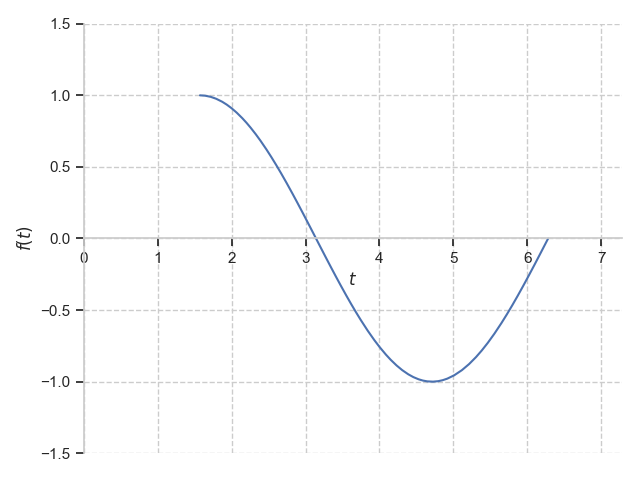
\includegraphics[scale=0.8]{odd_f(t).png}
    \captionsetup{skip=0pt}
    \caption{График $f(t)$ нечётной периодической функции}
    \label{Рис:23}
\end{figure}


\noindent Формулы для вычисления $a_n,\,a_0,\,b_n,\,c_n$ будут иметь вид:
\begin{align*}
    & a_n=\dfrac{4}{3\pi}\int\limits_{0.5\pi}^{2\pi}\sin{(t)}\cos{\left(\dfrac{4}{3}nt\right)}\,dt=\dfrac{2\left((4n-3)\left(\cos{\left(\dfrac{8\pi n}{3}\right)}+\sin{\left(\dfrac{2\pi n}{3}\right)}\right)-(4n+3)\left(\cos{\left(\dfrac{8\pi n}{3}\right)}-\sin{\left(\dfrac{2\pi n}{3}\right)}\right)\right)}{\pi (9-16n^2)}\\
    & b_n=\dfrac{4}{3\pi}\int\limits_{0.5\pi}^{2\pi}\sin{(t)}\sin{\left(\dfrac{4}{3}nt\right)}\,dt=\dfrac{2\left((4n-3)\left(\sin{\left(\dfrac{8\pi n}{3}\right)}-\cos{\left(\dfrac{2\pi n}{3}\right)}\right)-(4n+3)\left(\sin{\left(\dfrac{8\pi n}{3}\right)}+\cos{\left(\dfrac{2\pi n}{3}\right)}\right)\right)}{\pi (9-16n^2)}\\
    & c_n=\dfrac{2}{3\pi}\int\limits_{0.5\pi}^{2\pi}\sin{(t)}e^{-\frac{4i}{3}nt}\,dt=-\dfrac{2}{\pi(16n^2-9)}\left(3\left(i\sin{\left(\dfrac{8\pi n}{3}\right)}-\cos{\left(\dfrac{8\pi n}{3}\right)}\right)+4n\left(i\cos{\left(\dfrac{2\pi n}{3}\right)}+\sin{\left(\dfrac{2\pi n}{3}\right)}\right)\right)\\
    & a_0=\dfrac{4}{3\pi}\int\limits_{0.5\pi}^{2\pi}\sin{(t)}\,dt=-\dfrac{4}{3\pi}\cos{(t)}\bigg|_{0.5\pi}^{2\pi}=-\dfrac{4}{3\pi}
\end{align*}


\noindent Теперь составим $F_N(t)$ и $G_N(t)$:
\begin{align*}
    & F_N(t)=-\dfrac{2}{3\pi}+\sum_{n=1}^{N}\dfrac{2\left((4n-3)\left(\cos{\left(\dfrac{8\pi n}{3}\right)}+\sin{\left(\dfrac{2\pi n}{3}\right)}\right)-(4n+3)\left(\cos{\left(\dfrac{8\pi n}{3}\right)}-\sin{\left(\dfrac{2\pi n}{3}\right)}\right)\right)}{\pi (9-16n^2)}\cos{\left(\dfrac{4}{3}nt\right)}+\\
    & +\dfrac{2\left((4n-3)\left(\sin{\left(\dfrac{8\pi n}{3}\right)}-\cos{\left(\dfrac{2\pi n}{3}\right)}\right)-(4n+3)\left(\sin{\left(\dfrac{8\pi n}{3}\right)}+\cos{\left(\dfrac{2\pi n}{3}\right)}\right)\right)}{\pi (9-16n^2)}\sin{\left(\dfrac{4}{3}nt\right)}\\
    & G_N=\sum_{n=-N}^{N}-\dfrac{2e^{\frac{4i}{3}nt}}{\pi(16n^2-9)}\left(3\left(i\sin{\left(\dfrac{8\pi n}{3}\right)}-\cos{\left(\dfrac{8\pi n}{3}\right)}\right)+4n\left(i\cos{\left(\dfrac{2\pi n}{3}\right)}+\sin{\left(\dfrac{2\pi n}{3}\right)}\right)\right)
\end{align*}


\noindent С помощью написанной ранее программы вычислим значения коэффициентов при N=3
\begin{lstlisting}
a_3=0.0282942121052258
b_3=0.113176848420903
c_3=0.0141471060526129 - 0.0565884242104517*I
\end{lstlisting}


\noindent Построим графики $F_N(t)$, используя упрощенный код для нахождения частичной суммы ряда Фурье.
Функция $F_N(t)$ нарисована оранжевым цветом поверх заданной функции $f(t)$


\begin{figure}[!htb]
    \centering
    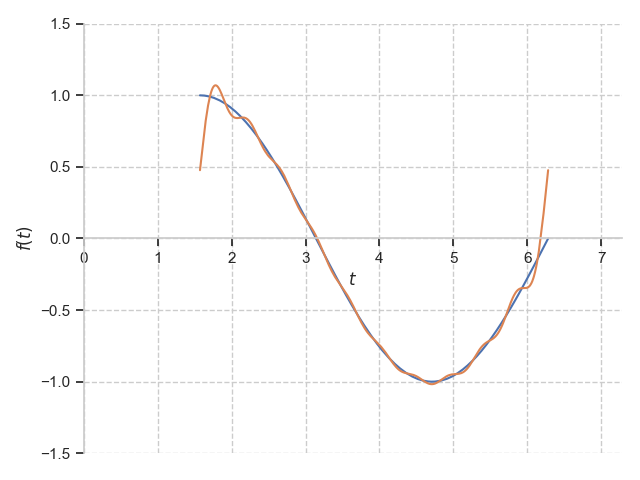
\includegraphics[scale=0.8]{fur_sin_n=10.png}
    \captionsetup{skip=0pt}
    \caption{График $F_N(t)$ нечётной периодической функции при N=10}
    \label{Рис:24}
\end{figure}
\newpage
\vspace*{10mm}
\begin{figure}[!htb]
    \centering
    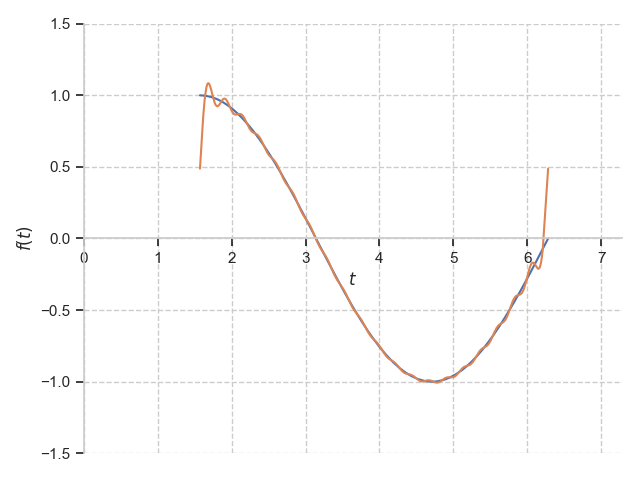
\includegraphics[scale=0.8]{fur_sin_n=20.png}
    \captionsetup{skip=0pt}
    \caption{График $F_N(t)$ нечётной периодической функции при N=20}
    \label{Рис:25}
\end{figure}
\begin{figure}[!htb]
    \centering
    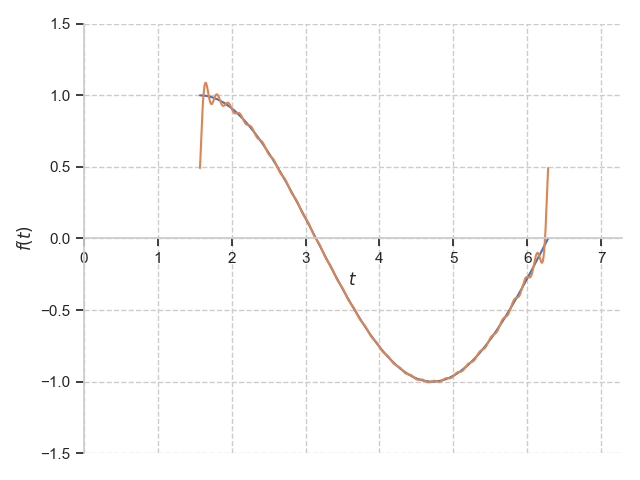
\includegraphics[scale=0.8]{fur_sin_n=30.png}
    \captionsetup{skip=0pt}
    \caption{График $F_N(t)$ нечётной периодической функции при N=30}
    \label{Рис:26}
\end{figure}
\newpage
\begin{figure}[!htb]
    \centering
    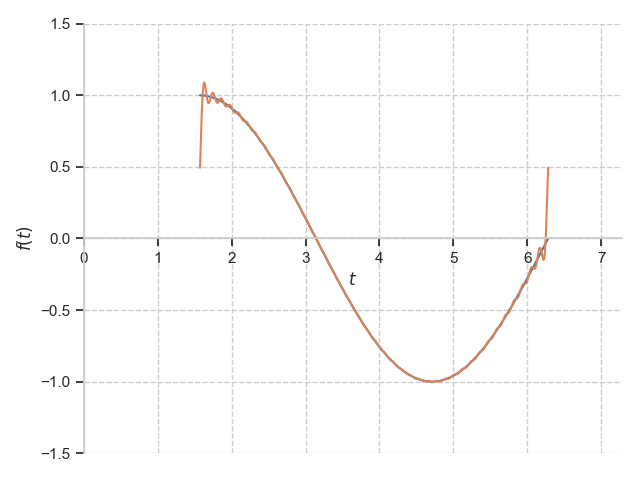
\includegraphics[scale=0.8]{fur_sin_n=40.png}
    \captionsetup{skip=0pt}
    \caption{График $F_N(t)$ нечётной периодической функции при N=40}
    \label{Рис:27}
\end{figure}
\begin{figure}[!htb]
    \centering
    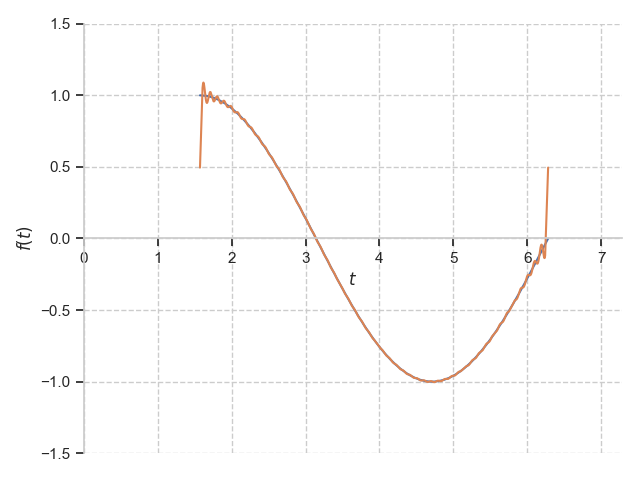
\includegraphics[scale=0.8]{fur_sin_n=50.png}
    \captionsetup{skip=0pt}
    \caption{График $F_N(t)$ нечётной периодической функции при N=50}
    \label{Рис:28}
\end{figure}


\noindent Наблюдаем такой же успех в аппроксимации функции, как и с графиком чётной периодической функции,
так как в сумме ряда Фурье преобладают синусы. Если бы период был $2\pi$, то графики $F_N(t)$ и $G_N(t)$
совпадали с $f(t)$, так как все $a_n$ занулились


\newpage
\noindent Проверим программой выполнение равенства Парсеваля. Результат для N=10:
\begin{lstlisting}
coeffs_sum=0.495154186636485    sqf_res=0.500000000000000
\end{lstlisting}


\noindent Результат для N=25:
\begin{lstlisting}
coeffs_sum=0.498011845838439    sqf_res=0.500000000000000
\end{lstlisting}


\noindent Результат для N=50:
\begin{lstlisting}
coeffs_sum=0.498996631466442    sqf_res=0.500000000000000
\end{lstlisting}


\noindent Результат для N=100:
\begin{lstlisting}
coeffs_sum=0.499495890594569    sqf_res=0.500000000000000
\end{lstlisting}


\noindent С увеличением N сумма коэффициентов приближается к результату интеграла, значит
существует стремление к равенству Парсеваля


\subsection{Ни чётная, ни нечётная периодическая функция}
\noindent Зададим следующую ни чётную, ни нечётную периодическую функцию:
$$f(t)=\cos{(t)}+t$$


\noindent Используя следующий код построим график функции $f(t)$:
\begin{lstlisting}[belowskip=-3mm]
f_t = not_even_or_odd_periodic_func(t)

def build_f_t():
    sp.plot((f_t, (t, gaps[0][0], gaps[-1][1])), 
            axis_center=(0, 0), xlim=(0, gap_end_val + 1), 
            ylim=(0, gap_end_val + 2), xlabel=r'$t$', 
            ylabel=r'$f(t)$')
build_f_t()
\end{lstlisting}
\begin{figure}[!htb]
    \centering
    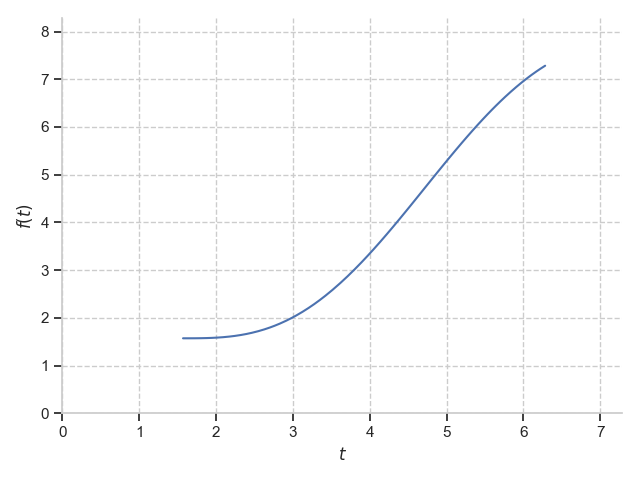
\includegraphics[scale=0.8]{evodd_f(t).png}
    \captionsetup{skip=0pt}
    \caption{График $f(t)$ ни чётной, ни нечётной периодической функции}
    \label{Рис:29}
\end{figure}


\newpage
\noindent Найдем формулы для вычисления коэффициентов $a_n,\,a_0,\,b_n,\,c_n$ и запишем $F_N(t)$ и $G_N(t)$:
\begin{align*}
    & a_n=\dfrac{4}{3\pi}\int\limits_{0.5\pi}^{2\pi}\left(\cos{\left(t\right)}+t\right)\cos{\left(\dfrac{4}{3}nt\right)}\,dt=\dfrac{1}{4{\pi}n^2\left(16n^2-9\right)}\left(\left(32n^3-24n^2\right)\sin\left(\dfrac{8{\pi}n}{3}\right)+\left(32n^3+24n^2\right)\sin\left(\dfrac{8{\pi}n}{3}\right)+\right.\\
    & +\left(24n^2-32n^3\right)\cos\left(\dfrac{2{\pi}n}{3}\right)+\left(32n^3+24n^2\right)\cos\left(\dfrac{2{\pi}n}{3}\right)+\left(128{\pi}n^3-72{\pi}n\right)\sin\left(\dfrac{8{\pi}n}{3}\right)+\left(48n^2-27\right)\cos\left(\dfrac{8{\pi}n}{3}\right)\\
    & \left.+\left(18{\pi}n-32{\pi}n^3\right)\sin\left(\dfrac{2{\pi}n}{3}\right)+\left(27-48n^2\right)\cos\left(\dfrac{2{\pi}n}{3}\right)\right)\\
    & b_n=\dfrac{4}{3\pi}\int\limits_{0.5\pi}^{2\pi}\left(\cos{\left(t\right)}+t\right)\sin{\left(\dfrac{4}{3}nt\right)}\,dt=-\dfrac{1}{4{\pi}n^2\left(16n^2-9\right)}\left(\left(32n^3-24n^2\right)\cos\left(\dfrac{8{\pi}n}{3}\right)+\left(32n^3+24n^2\right)\cos\left(\dfrac{8{\pi}n}{3}\right)+\right.\\
    & +\left(32n^3-24n^2\right)\cos\left(\dfrac{2{\pi}n}{3}\right)+\left(-32n^3-24n^2\right)\sin\left(\dfrac{2{\pi}n}{3}\right)+\left(27-48n^2\right)\sin\left(\dfrac{8{\pi}n}{3}\right)+\left(128{\pi}n^3-72{\pi}n\right)\cos\left(\dfrac{8{\pi}n}{3}\right)+\\
    & \left.+\left(48n^2-27\right)\sin\left(\dfrac{2{\pi}n}{3}\right)+\left(18{\pi}n-32{\pi}n^3\right)\cos\left(\dfrac{2{\pi}n}{3}\right)\right)\\
    & c_n=\dfrac{2}{3\pi}\int\limits_{0.5\pi}^{2\pi}\left(\cos{(t)}+t\right)e^{-\frac{4i}{3}nt}\,dt=\dfrac{1}{{4{\pi}n^2\left(16n^2-9\right)}}\left(\left(32n^3-24n^2\right)\sin\left(\dfrac{8{\pi}n}{3}\right)+\left(24in^2-32in^3\right)\cos\left(\dfrac{8{\pi}n}{3}\right)+\right.\\
    & +\left(32n^3+24n^2\right)\sin\left(\dfrac{8{\pi}n}{3}\right)+\left(-32in^3-24in^2\right)\cos\left(\dfrac{8{\pi}n}{3}\right)+\left(24n^2-32n^3\right)\cos\left(\dfrac{2{\pi}n}{3}\right)+\\
    & +\left(24in^2-32in^3\right)\sin\left(\dfrac{2{\pi}n}{3}\right)+\left(32n^3+24n^2\right)\cos\left(\dfrac{2{\pi}n}{3}\right)+\left(32in^3+24in^2\right)\sin\left(\dfrac{2{\pi}n}{3}\right)+\\
    & +\left(128{\pi}n^3+48in^2-72{\pi}n-27i\right)\sin\left(\dfrac{8{\pi}n}{3}\right)+\left(-128i{\pi}n^3+48n^2+72i{\pi}n-27\right)\cos\left(\dfrac{8{\pi}n}{3}\right)+\\
    & \left.+\left(-32{\pi}n^3-48in^2+18{\pi}n+27i\right)\sin\left(\dfrac{2{\pi}n}{3}\right)+\left(32i{\pi}n^3-48n^2-18i{\pi}n+27\right)\cos\left(\dfrac{2{\pi}n}{3}\right)\right)\\
    & a_0=\dfrac{4}{3\pi}\int\limits_{0.5\pi}^{2\pi}\left(\cos{\left(t\right)}+t\right)\,dt=\dfrac{4}{3\pi}\left(\,\int\limits_{0.5\pi}^{2\pi}\cos{(t)}\,dt+\int\limits_{0.5\pi}^{2\pi}t\,dt\right)=\dfrac{4}{3\pi}\left(\sin{(t)}+\dfrac{t^2}{2}\right)\bigg|_{0.5\pi}^{2\pi}=\dfrac{15\pi^2-8}{6\pi}\\
    & F_N(t)=\dfrac{15\pi^2-8}{12\pi}+\sum_{n=1}^{N}\dfrac{1}{4{\pi}n^2\left(16n^2-9\right)}\left(\left(\left(32n^3-24n^2\right)\sin\left(\dfrac{8{\pi}n}{3}\right)+\left(32n^3+24n^2\right)\sin\left(\dfrac{8{\pi}n}{3}\right)+\right.\right.\\
    & +\left(24n^2-32n^3\right)\cos\left(\dfrac{2{\pi}n}{3}\right)+\left(32n^3+24n^2\right)\cos\left(\dfrac{2{\pi}n}{3}\right)+\left(128{\pi}n^3-72{\pi}n\right)\sin\left(\dfrac{8{\pi}n}{3}\right)+\\
    & \left.+\left(48n^2-27\right)\cos\left(\dfrac{8{\pi}n}{3}\right)+\left(18{\pi}n-32{\pi}n^3\right)\sin\left(\dfrac{2{\pi}n}{3}\right)+\left(27-48n^2\right)\cos\left(\dfrac{2{\pi}n}{3}\right)\right)\cos{\left(\dfrac{4}{3}nt\right)}+\\
    & -\left(\left(32n^3-24n^2\right)\cos\left(\dfrac{8{\pi}n}{3}\right)+\left(32n^3+24n^2\right)\cos\left(\dfrac{8{\pi}n}{3}\right)+\left(32n^3-24n^2\right)\cos\left(\dfrac{2{\pi}n}{3}\right)\right.+\\
    & +\left(-32n^3-24n^2\right)\sin\left(\dfrac{2{\pi}n}{3}\right)+\left(27-48n^2\right)\sin\left(\dfrac{8{\pi}n}{3}\right)+\left(128{\pi}n^3-72{\pi}n\right)\cos\left(\dfrac{8{\pi}n}{3}\right)+\\
    & \left.\left.+\left(48n^2-27\right)\sin\left(\dfrac{2{\pi}n}{3}\right)+\left(18{\pi}n-32{\pi}n^3\right)\cos\left(\dfrac{2{\pi}n}{3}\right)\right)\sin{\left(\dfrac{4}{3}nt\right)}\right)\\
    & G_N=\sum_{n=-N}^{N}\dfrac{1}{4{\pi}n^2\left(16n^2-9\right)}\left(\left(32n^3-24n^2\right)\sin\left(\dfrac{8{\pi}n}{3}\right)+\left(24in^2-32in^3\right)\cos\left(\dfrac{8{\pi}n}{3}\right)+\right.\\
    & +\left(32n^3+24n^2\right)\sin\left(\dfrac{8{\pi}n}{3}\right)+\left(-32in^3-24in^2\right)\cos\left(\dfrac{8{\pi}n}{3}\right)+\left(24n^2-32n^3\right)\cos\left(\dfrac{2{\pi}n}{3}\right)+\\
    & +\left(24in^2-32in^3\right)\sin\left(\dfrac{2{\pi}n}{3}\right)+\left(32n^3+24n^2\right)\cos\left(\dfrac{2{\pi}n}{3}\right)+\left(32in^3+24in^2\right)\sin\left(\dfrac{2{\pi}n}{3}\right)+\\
    & +\left(128{\pi}n^3+48in^2-72{\pi}n-27i\right)\sin\left(\dfrac{8{\pi}n}{3}\right)+\left(-128i{\pi}n^3+48n^2+72i{\pi}n-27\right)\cos\left(\dfrac{8{\pi}n}{3}\right)+\\
    & \left.+\left(-32{\pi}n^3-48in^2+18{\pi}n+27i\right)\sin\left(\dfrac{2{\pi}n}{3}\right)+\left(32i{\pi}n^3-48n^2-18i{\pi}n+27\right)\cos\left(\dfrac{2{\pi}n}{3}\right)\right)e^{\frac{4i}{3}nt}
\end{align*}


\newpage
\noindent Вычислим программно значения коэффициентов при N=3:
\begin{lstlisting}
a_3=0.0282942121052258
b_3=-0.613176848420903
c_3=0.0141471060526129 + 0.306588424210452*I
\end{lstlisting}


\noindent Построим графики $F_N(t)$ для различных значений N. Примеры использования кода были
приведены ранее, здесь также используется упрощенный алгоритм для одной функции на одном интервале.
Оранжевым цветом нарисована $F_N(t)$ поверх функции $f(t)$
\begin{figure}[!htb]
    \centering
    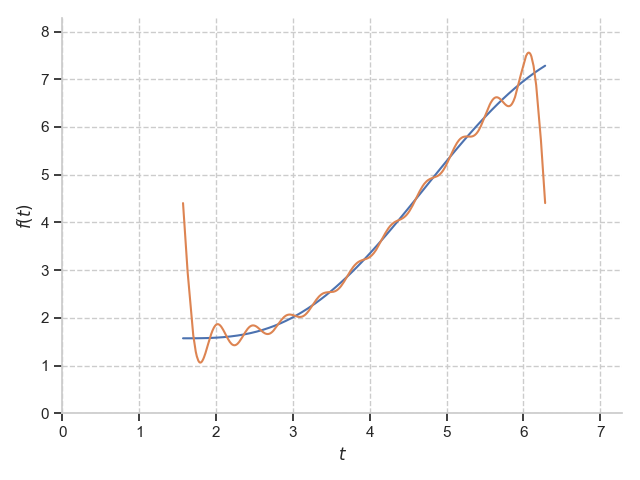
\includegraphics[scale=0.8]{fur_evodd_n=10.png}
    \captionsetup{skip=0pt}
    \caption{График $F_N(t)$ ни чётной, ни нечётной периодической функции при N=10}
    \label{Рис:30}
\end{figure}
\begin{figure}[!htb]
    \centering
    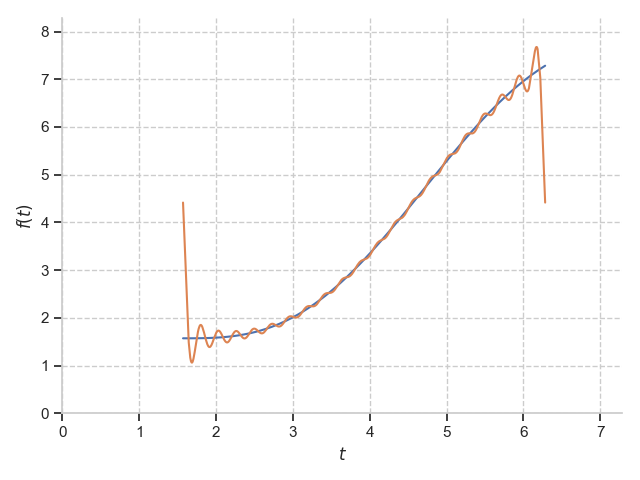
\includegraphics[scale=0.8]{fur_evodd_n=20.png}
    \captionsetup{skip=0pt}
    \caption{График $F_N(t)$ ни чётной, ни нечётной периодической функции при N=20}
    \label{Рис:31}
\end{figure}
\newpage
\vspace*{10mm}
\begin{figure}[!htb]
    \centering
    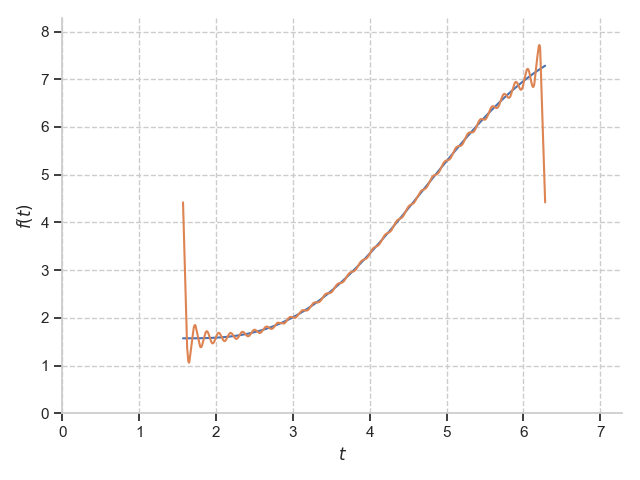
\includegraphics[scale=0.8]{fur_evodd_n=30.png}
    \captionsetup{skip=0pt}
    \caption{График $F_N(t)$ ни чётной, ни нечётной периодической функции при N=30}
    \label{Рис:32}
\end{figure}
\begin{figure}[!htb]
    \centering
    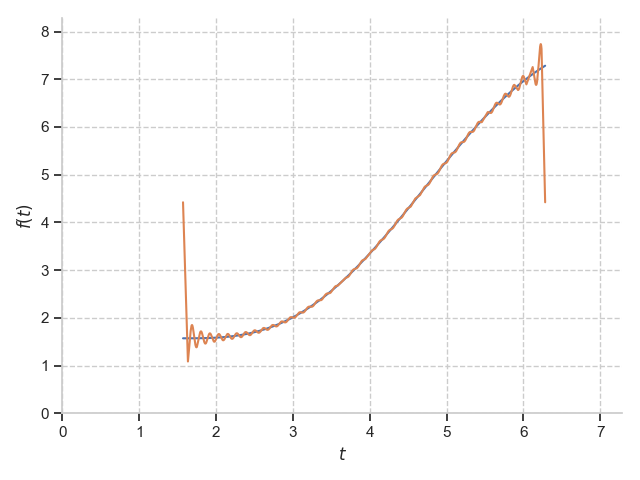
\includegraphics[scale=0.8]{fur_evodd_n=40.png}
    \captionsetup{skip=0pt}
    \caption{График $F_N(t)$ ни чётной, ни нечётной периодической функции при N=40}
    \label{Рис:33}
\end{figure}
\newpage
\begin{figure}[!htb]
    \centering
    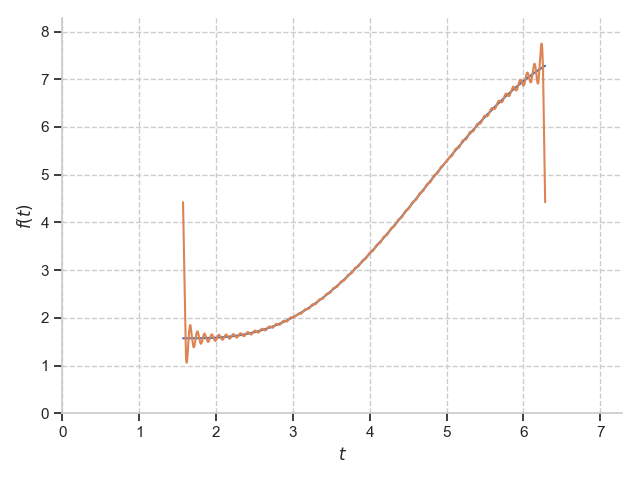
\includegraphics[scale=0.8]{fur_evodd_n=50.png}
    \captionsetup{skip=0pt}
    \caption{График $F_N(t)$ ни чётной, ни нечётной периодической функции при N=50}
    \label{Рис:34}
\end{figure}


\noindent Снова наблюдаем как ряд Фурье хорошо описывает заданную функцию. В данном случае
в сумме ряда Фурье достаточно и синусов и косинусов, что позволяет описать ни чётную, ни 
нечётную функцию. Преобладание синусов приведет к графику, похожему на синусоиду, а косинусов
на косинусоиду


\noindent Проверим выполнение равенства Парсеваля при N=10, 25, 50, 100 соответственно:
\begin{lstlisting}
coeffs_sum=17.3721304758656
coeffs_sum=17.4647269560923
coeffs_sum=17.4968192131263
coeffs_sum=17.5131052270956
sqf_res=17.5295542168181
\end{lstlisting}


\noindent При N$\geq$100 сумма коэффициентов близка к значению
интеграла функции, следовательно сумма коэффициентов стремится к равенству Парсеваля


\newpage
\section{Комплексная функция}
\subsection{Комплекснозначная функция \texorpdfstring{$f:\mathbf{R}\rightarrow\mathbf{C}$}{Lg}}
\noindent Зададим числа $R,\,T>0$. Пусть $R=2,\,T=2\pi$. Рассмотрим следующую функцию:
$$
\text{Re}\,f(t)=
\begin{cases}
    2, & t\in[\,-\frc{\pi}{4},\frc{\pi}{4}\,),\\
    4-\frc{8t}{\pi}, & t\in[\,\frc{\pi}{4},\frc{3\pi}{4}\,),\\
    -2, & t\in[\,\frc{3\pi}{4},\frc{5\pi}{4}\,),\\
    -12+\frc{8t}{\pi}, & t\in[\,\frc{5\pi}{4},\frc{7\pi}{4}\,),
\end{cases}
\,\,\,\,\,\,\,\,\,\,\,\,\,\,\,\,
\text{Im}\,f(t)=
\begin{cases}
    \frc{8t}{\pi}, & t\in[\,-\frc{\pi}{4},\frc{\pi}{4}\,),\\
    2, & t\in[\,\frc{\pi}{4},\frc{3\pi}{4}\,),\\
    8-\frc{8t}{\pi}, & t\in[\,\frc{3\pi}{4},\frc{5\pi}{4}\,),\\
    -2, & t\in[\,\frc{5\pi}{4},\frc{7\pi}{4}\,),
\end{cases}
$$


\noindent Прежде чем строить график $f(t)$ на языке программирования python с
использованием библиотеки sympy, познакомимся с файлом static.py для задания 2:


\begin{lstlisting}
import sympy as sp

R = 2
T = 2 * sp.pi
    
pN = 25
N = 3
N_1 = 1
N_2 = 2
N_3 = 3
N_4 = 10
    
t = sp.Symbol('t')
    
point_common = T / 8
    
point_1 = -point_common
point_1_val = float(point_1.evalf())
    
point_2 = point_common
point_2_val = float(point_2.evalf())
    
point_3 = 3 * point_common
point_3_val = float(point_3.evalf())
    
point_4 = 5 * point_common
point_4_val = float(point_4.evalf())
    
point_5 = 7 * point_common
point_5_val = float(point_5.evalf())
    
gap_1 = [point_1, point_2]
gap_2 = [point_2, point_3]
gap_3 = [point_3, point_4]
gap_4 = [point_4, point_5]
gaps = [gap_1, gap_2, gap_3, gap_4]
    
gap_len = gap_4[1] - gap_1[0]
gap_len_val = float(gap_len.evalf())
    
# can not compare expressions with a
# variable like "t" so bad code here
def gap_1_cfunc(t):
    return R + (8 * R * t / T) * 1j
    
def gap_2_cfunc(t):
    return 2 * R - (8 * R * t / T) + R * 1j
    
def gap_3_cfunc(t):
    return -R + (4 * R - (8 * R * t / T)) * 1j
    
def gap_4_cfunc(t):
    return -6 * R + (8 * R * t / T) - R * 1j
\end{lstlisting}


\noindent Аналогично принципу из задания 1 из этого файла будут импортироваться все
необходимые данные для работы с рядом Фурье и построения графиков. Я задал функции,
объединив действительные и мнимые части на одинаковых интервалах по типу $z=a+ib$ и
упростил выражения


\newpage
\noindent Пример кода для построения параметрического графика комплекснозначной функции:
\begin{lstlisting}[belowskip=-3mm]
f_c_1, f_c_2, f_c_3, f_c_4 = gap_1_cfunc(t), gap_2_cfunc(t), gap_3_cfunc(t), gap_4_cfunc(t)
def build_f_t():
    sp.plot_parametric((sp.re(f_c_1), sp.im(f_c_1), (t, gaps[0][0], gaps[0][1])),
                       (sp.re(f_c_2), sp.im(f_c_2), (t, gaps[1][0], gaps[1][1])),
                       (sp.re(f_c_3), sp.im(f_c_3), (t, gaps[2][0], gaps[2][1])),
                       (sp.re(f_c_4), sp.im(f_c_4), (t, gaps[3][0], gaps[3][1])), 
                       xlabel=r'Re$(t)$', ylabel=r'Im$(t)$')
\end{lstlisting}
\begin{figure}[!htb]
    \centering
    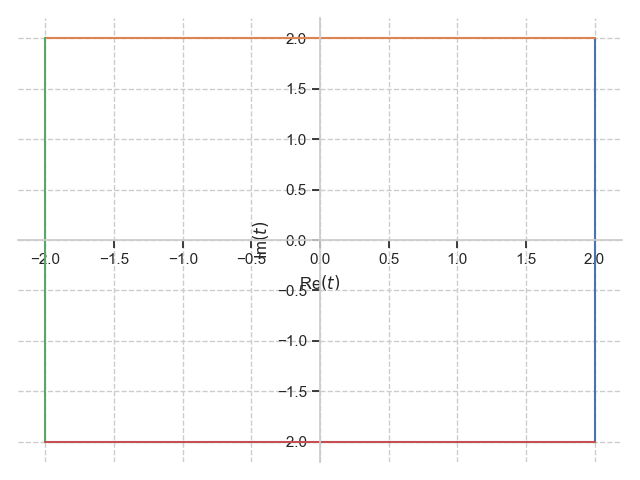
\includegraphics[scale=0.8]{cf(t).png}
    \captionsetup{skip=0pt}
    \caption{Параметрический график $f(t)$ комплекснозначной функции}
    \label{Рис:35}
\end{figure}


\noindent Запишем коэффициент $c_n$:
\begin{align*}
    & c_n =\dfrac{1}{2\pi}\int\limits_{h}^{h+T}f(t)e^{-int}\,dt=\dfrac{1}{2\pi}\left(\int\limits_{-\frac{\pi}{4}}^{\frac{\pi}{4}}\left(2+\dfrac{8t}{\pi}\right)e^{-int}\,dt+\int\limits_{\frac{\pi}{4}}^{\frac{3\pi}{4}}\left(6-\dfrac{8t}{\pi}\right)e^{-int}\,dt+\right.\\
    &\left. \int\limits_{\frac{3\pi}{4}}^{\frac{5\pi}{4}}\left(6-\dfrac{8t}{\pi}\right)e^{-int}\,dt+\int\limits_{\frac{5\pi}{4}}^{\frac{7\pi}{4}}\left(-14+\dfrac{8t}{\pi}\right)e^{-int}\,dt\right)
\end{align*}


\noindent Рассмотрим отдельно интеграл функции $2+\frc{8t}{\pi}$ на промежутке $[-\frc{\pi}{4}, \frc{\pi}{4})$:
\begin{align}
    & \int\limits_{-\frac{\pi}{4}}^{\frac{\pi}{4}}\left(2+\dfrac{8t}{\pi}\right)e^{-int}\,dt=
    \begin{bmatrix}
        u=2+\frc{8t}{\pi} &v=\int e^{-int}\,dt\\
        du=\frc{8}{\pi}\,dt &dv=e^{-int}\,dt
    \end{bmatrix},\\
    & v=\int e^{-int}\,dt=
    \begin{bmatrix}
        x=-int\\
        dx=-in\,dt\\
        dt=\frc{i}{n}\,dx
    \end{bmatrix}=
    \dfrac{i}{n}\int e^{x}\,dx=\dfrac{i}{n}e^{x}=\dfrac{i}{n}e^{-int},\\
    & \int u\,dv=uv-\int v\,du\Rightarrow (1)=\dfrac{i}{n}\left(2+\dfrac{8t}{\pi}\right)e^{-int}\bigg|_{-\frac{\pi}{4}}^{\frac{\pi}{4}}-\dfrac{8i}{\pi n}\int\limits_{-\frac{\pi}{4}}^{\frac{\pi}{4}}e^{-int}\,dt,\\
    & \dfrac{i}{n}\left(2+\dfrac{8t}{\pi}\right)e^{-int}\bigg|_{-\frac{\pi}{4}}^{\frac{\pi}{4}}=\dfrac{i}{n}\left(\left(2+\dfrac{8\cdot\frc{\pi}{4}}{\pi}\right)e^{-\frac{\pi}{4}in}-\left(2+\dfrac{8\cdot\left(-\frc{\pi}{4}\right)}{\pi}\right)e^{\frac{\pi}{4}in}\right)=\dfrac{4i}{n}e^{-\frac{\pi}{4}in},\\
    & -\dfrac{8i}{\pi n}\int\limits_{-\frac{\pi}{4}}^{\frac{\pi}{4}}e^{-int}\,dt=-\dfrac{8i}{\pi n}\cdot\dfrac{i}{n}e^{-int}\bigg|_{-\frac{\pi}{4}}^{\frac{\pi}{4}}=\dfrac{8}{\pi n^2}e^{-int}\bigg|_{-\frac{\pi}{4}}^{\frac{\pi}{4}}=\dfrac{8}{\pi n^2}\left(e^{-\frac{\pi}{4}in}-e^{\frac{\pi}{4}in}\right),\\
    & (1)=(4)+(5)=\dfrac{4i}{n}e^{-\frac{\pi}{4}in}+\dfrac{8}{\pi n^2}\left(e^{-\frac{\pi}{4}in}-e^{\frac{\pi}{4}in}\right)=\dfrac{4}{n}\left(ie^{-\frac{\pi}{4}in}+\dfrac{2}{\pi n}\left(e^{-\frac{\pi}{4}in}-e^{\frac{\pi}{4}in}\right)\right)
\end{align}


\noindent Остальные интегралы решаются аналогичным способом, поэтому я приведу неполное решение для них:
\begin{align*}
    & \int\limits_{\frac{\pi}{4}}^{\frac{3\pi}{4}}\left(6-\dfrac{8t}{\pi}\right)e^{-int}\,dt=\dfrac{i}{n}\left(6-\dfrac{8t}{\pi}\right)e^{-int}\bigg|_{\frac{\pi}{4}}^{\frac{3\pi}{4}}-\dfrac{8}{\pi n^2}e^{-int}\bigg|_{\frac{\pi}{4}}^{\frac{3\pi}{4}}=-\dfrac{4}{n}\left(ie^{-\frac{\pi}{4}in}+\dfrac{2}{\pi n}\left(e^{-\frac{3\pi}{4}in}-e^{-\frac{\pi}{4}in}\right)\right)\\
    & \int\limits_{\frac{3\pi}{4}}^{\frac{5\pi}{4}}\left(6-\dfrac{8t}{\pi}\right)e^{-int}\,dt=\dfrac{i}{n}\left(6-\dfrac{8t}{\pi}\right)e^{-int}\bigg|_{\frac{3\pi}{4}}^{\frac{5\pi}{4}}-\dfrac{8}{\pi n^2}e^{-int}\bigg|_{\frac{3\pi}{4}}^{\frac{5\pi}{4}}=-\dfrac{4}{n}\left(ie^{-\frac{5\pi}{4}in}+\dfrac{2}{\pi n}\left(e^{-\frac{5\pi}{4}in}-e^{-\frac{3\pi}{4}in}\right)\right)\\
    & \int\limits_{\frac{5\pi}{4}}^{\frac{7\pi}{4}}\left(-14+\dfrac{8t}{\pi}\right)e^{-int}\,dt=\dfrac{i}{n}\left(-14+\dfrac{8t}{\pi}\right)e^{-int}\bigg|_{\frac{5\pi}{4}}^{\frac{7\pi}{4}}+\dfrac{8}{\pi n^2}e^{-int}\bigg|_{\frac{5\pi}{4}}^{\frac{7\pi}{4}}=\dfrac{4}{n}\left(ie^{-\frac{5\pi}{4}in}+\dfrac{2}{\pi n}\left(e^{-\frac{7\pi}{4}in}-e^{-\frac{5\pi}{4}in}\right)\right)
\end{align*}


\noindent Суммируем все вычисленные интегралы и упростим выражение:
\begin{align*}
    & \dfrac{4}{n}\left(ie^{-\frac{\pi}{4}in}+\dfrac{2}{\pi n}\left(e^{-\frac{\pi}{4}in}-e^{\frac{\pi}{4}in}\right)\right)-\dfrac{4}{n}\left(ie^{-\frac{\pi}{4}in}+\dfrac{2}{\pi n}\left(e^{-\frac{3\pi}{4}in}-e^{-\frac{\pi}{4}in}\right)\right)-\dfrac{4}{n}\left(ie^{-\frac{5\pi}{4}in}+\dfrac{2}{\pi n}\left(e^{-\frac{5\pi}{4}in}-e^{-\frac{3\pi}{4}in}\right)\right)+\\
    & +\dfrac{4}{n}\left(ie^{-\frac{5\pi}{4}in}+\dfrac{2}{\pi n}\left(e^{-\frac{7\pi}{4}in}-e^{-\frac{5\pi}{4}in}\right)\right)=\dfrac{4}{n}\left(ie^{-\frac{\pi}{4}in}+\dfrac{2}{\pi n}\left(e^{-\frac{\pi}{4}in}-e^{\frac{\pi}{4}in}\right)-ie^{-\frac{\pi}{4}in}-\dfrac{2}{\pi n}\left(e^{-\frac{3\pi}{4}in}-e^{-\frac{\pi}{4}in}\right)+\right.\\
    & \left. -ie^{-\frac{5\pi}{4}in}-\dfrac{2}{\pi n}\left(e^{-\frac{5\pi}{4}in}-e^{-\frac{3\pi}{4}in}\right)+ie^{-\frac{5\pi}{4}in}+\dfrac{2}{\pi n}\left(e^{-\frac{7\pi}{4}in}-e^{-\frac{5\pi}{4}in}\right)\right)=\dfrac{4}{n}\cdot\dfrac{2}{\pi n}\left(e^{-\frac{\pi}{4}in}-e^{\frac{\pi}{4}in}-e^{-\frac{3\pi}{4}in}+e^{-\frac{\pi}{4}in}+\right.\\
    & \left. -e^{-\frac{5\pi}{4}in}+e^{-\frac{3\pi}{4}in}+e^{-\frac{7\pi}{4}in}-e^{-\frac{5\pi}{4}in}\right)=\dfrac{8}{\pi n^2}\left(2\left(e^{-\frac{\pi}{4}in}-e^{-\frac{5\pi}{4}in}\right)+e^{-\frac{7\pi}{4}in}-e^{\frac{\pi}{4}in}\right)
\end{align*}


\noindent Тогда коэффициент $c_n$ будет иметь вид:
\begin{align*}
    & c_n=\dfrac{1}{2\pi}\cdot\dfrac{8}{\pi n^2}\left(2\left(e^{-\frac{\pi}{4}in}-e^{-\frac{5\pi}{4}in}\right)+e^{-\frac{7\pi}{4}in}-e^{\frac{\pi}{4}in}\right)=\dfrac{4}{\left(\pi n\right)^2}\left(2\left(e^{-\frac{\pi}{4}in}-e^{-\frac{5\pi}{4}in}\right)+e^{-\frac{7\pi}{4}in}-e^{\frac{\pi}{4}in}\right)
\end{align*}


\noindent Получим следующий ряд Фурье $G_N(t)$:
\begin{align*}
    & G_N(t)=\sum_{n=-N}^{N}\dfrac{4e^{int}}{\left(\pi n\right)^2}\left(2\left(e^{-\frac{\pi}{4}in}-e^{-\frac{5\pi}{4}in}\right)+e^{-\frac{7\pi}{4}in}-e^{\frac{\pi}{4}in}\right)
\end{align*}


\noindent Вычислим коэффициенты $c_0,\,c_1,\,c_2$:
\begin{align*}
    & c_0=\dfrac{1}{2\pi}\left(\int\limits_{-\frac{\pi}{4}}^{\frac{\pi}{4}}\left(2+\dfrac{8t}{\pi}\right)\,dt+\int\limits_{\frac{\pi}{4}}^{\frac{3\pi}{4}}\left(6-\dfrac{8t}{\pi}\right)\,dt+\int\limits_{\frac{3\pi}{4}}^{\frac{5\pi}{4}}\left(6-\dfrac{8t}{\pi}\right)\,dt+\int\limits_{\frac{5\pi}{4}}^{\frac{7\pi}{4}}\left(-14+\dfrac{8t}{\pi}\right)\,dt\right)=\dfrac{1}{2\pi}\left(\left(2t+\dfrac{8t^2}{2\pi}\right)\bigg|_{-\frac{\pi}{4}}^{\frac{\pi}{4}}+\right.\\
    & \left. +\left(6t-\dfrac{8t^2}{2\pi}\right)\bigg|_{\frac{\pi}{4}}^{\frac{3\pi}{4}}+\left(6t-\dfrac{8t^2}{2\pi}\right)\bigg|_{\frac{3\pi}{4}}^{\frac{5\pi}{4}}+\left(-14t+\dfrac{8t^2}{2\pi}\right)\bigg|_{\frac{5\pi}{4}}^{\frac{7\pi}{4}}\right)=\dfrac{1}{2\pi}\left(\pi+\pi-\pi-\pi\right)=0\\
    & c_1=\dfrac{4}{\pi^2}\left(2\left(e^{-\frac{\pi}{4}i}-e^{-\frac{5\pi}{4}i}\right)+e^{-\frac{7\pi}{4}i}-e^{\frac{\pi}{4}i}\right)=\dfrac{8}{\pi^2}\left(e^{-\frac{\pi}{4}i}-e^{\frac{3\pi}{4}i}\right)\\
    & c_2=\dfrac{1}{\pi^2}\left(2\left(e^{-\frac{\pi}{2}i}-e^{-\frac{5\pi}{2}i}\right)+e^{-\frac{7\pi}{2}i}-e^{\frac{\pi}{2}i}\right)=0
\end{align*}


\noindent Воспользуемся ранее написанной программой и вычислим $c_3$:
\begin{lstlisting}
c_3=-1.24943987955415e-17 + 8.74607915687906e-17*I
\end{lstlisting}


\noindent Далее построим параметрические графики $G_N(t)$ для N=1, 2, 3, 10. $G_N(t)$
нарисована фиолетовым цветом поверх параметрического графика $f(t)$


\newpage
\vspace*{10mm}
\begin{figure}[!htb]
    \centering
    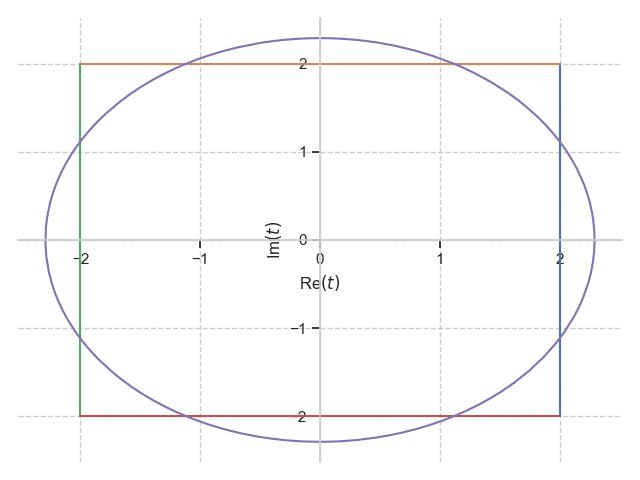
\includegraphics[scale=0.8]{fur_cf_n=1.png}
    \captionsetup{skip=0pt}
    \caption{График $G_N(t)$ комплекснозначной функции при N=1}
    \label{Рис:36}
\end{figure}
\begin{figure}[!htb]
    \centering
    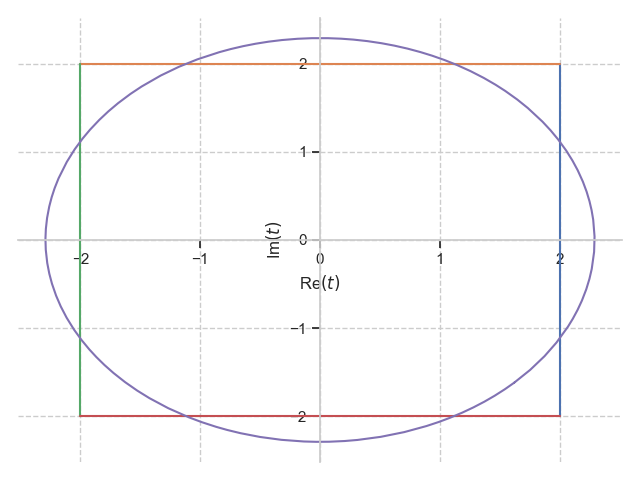
\includegraphics[scale=0.8]{fur_cf_n=2.png}
    \captionsetup{skip=0pt}
    \caption{График $G_N(t)$ комплекснозначной функции при N=2}
    \label{Рис:37}
\end{figure}
\newpage
\begin{figure}[!htb]
    \centering
    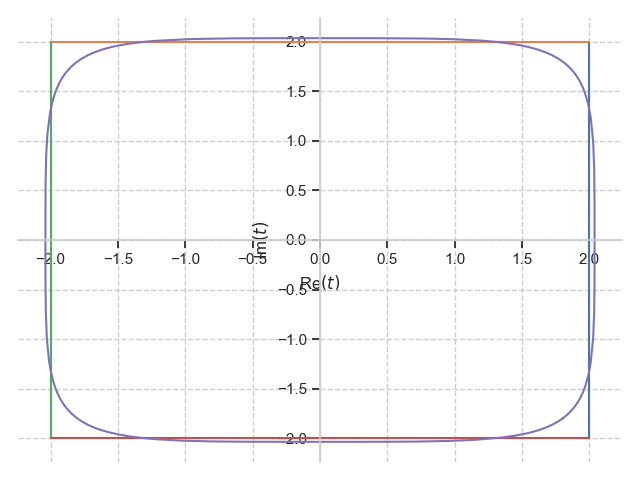
\includegraphics[scale=0.8]{fur_cf_n=3.png}
    \captionsetup{skip=0pt}
    \caption{График $G_N(t)$ комплекснозначной функции при N=3}
    \label{Рис:38}
\end{figure}
\begin{figure}[!htb]
    \centering
    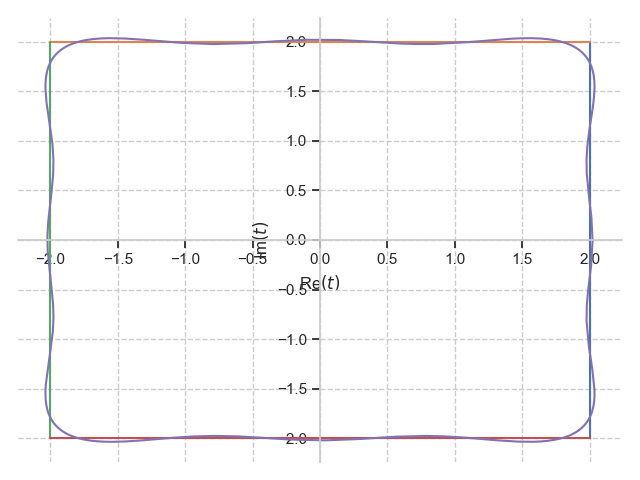
\includegraphics[scale=0.8]{fur_cf_n=10.png}
    \captionsetup{skip=0pt}
    \caption{График $G_N(t)$ комплекснозначной функции при N=10}
    \label{Рис:39}
\end{figure}


\noindent Как видим, при N$<$3 график $G_N(t)$ напоминает эллипс, а
при N$\geq3$ стремится к квадрату, то есть к функции $f(t)$


\noindent Далее построим графики Re$\,f(t)$, Im$\,f(t)$ и графики Re$\,G_N(t)$, Im$\,G_N(t)$ для N=1, 2, 3, 10.
Пример кода для построения графика Re$\,G_N(t)$:
\begin{lstlisting}
funcs = [gap_1_cfunc, gap_2_cfunc, gap_3_cfunc, gap_4_cfunc]
def build_Re_G_N(N):
    G_N = calc_G_N_generic(N, gaps, funcs)
    sp.plot((sp.re(G_N), (t, gaps[0][0], gaps[-1][1])),
            xlabel=r'$t$', ylabel=r'Re$(G_{N}(t))$')
build_Re_G_N(N_1)
\end{lstlisting}


\newpage
\vspace*{10mm}
\begin{figure}[!htb]
    \centering
    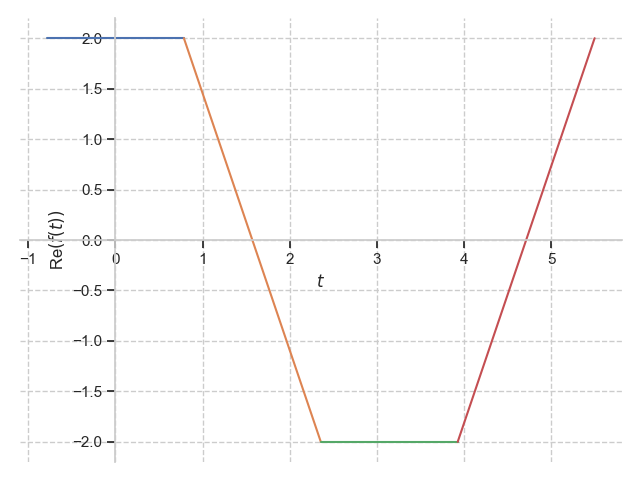
\includegraphics[scale=0.8]{re_cf(t).png}
    \captionsetup{skip=0pt}
    \caption{График Re$\,f(t)$ комплекснозначной функции}
    \label{Рис:40}
\end{figure}
\begin{figure}[!htb]
    \centering
    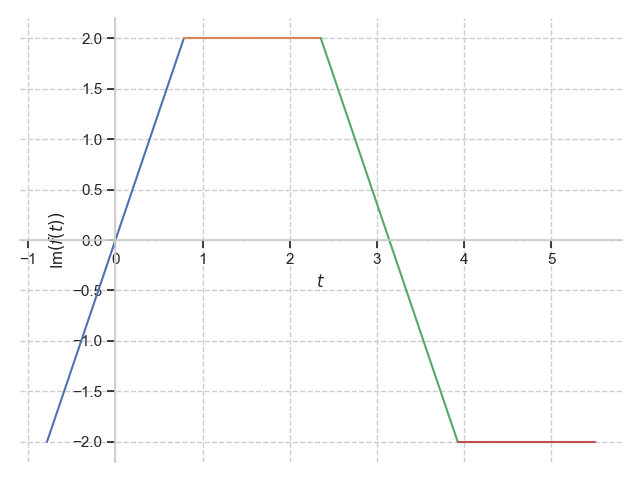
\includegraphics[scale=0.8]{im_cf(t).png}
    \captionsetup{skip=0pt}
    \caption{График Im$\,f(t)$ комплекснозначной функции}
    \label{Рис:41}
\end{figure}
\newpage
\vspace*{10mm}
\begin{figure}[!htb]
    \centering
    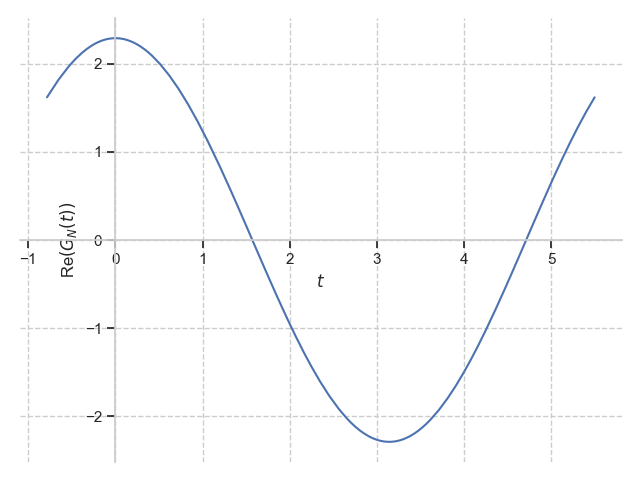
\includegraphics[scale=0.8]{fourier_re_cfunc_n=1.png}
    \captionsetup{skip=0pt}
    \caption{График Re$\,G_N(t)$ комплекснозначной функции при N=1}
    \label{Рис:42}
\end{figure}
\begin{figure}[!htb]
    \centering
    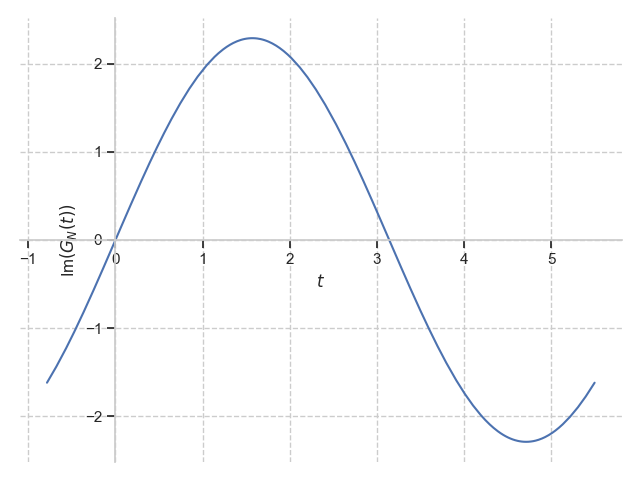
\includegraphics[scale=0.8]{fourier_im_cfunc_n=1.png}
    \captionsetup{skip=0pt}
    \caption{График Im$\,G_N(t)$ комплекснозначной функции при N=1}
    \label{Рис:43}
\end{figure}
\newpage
\vspace*{10mm}
\begin{figure}[!htb]
    \centering
    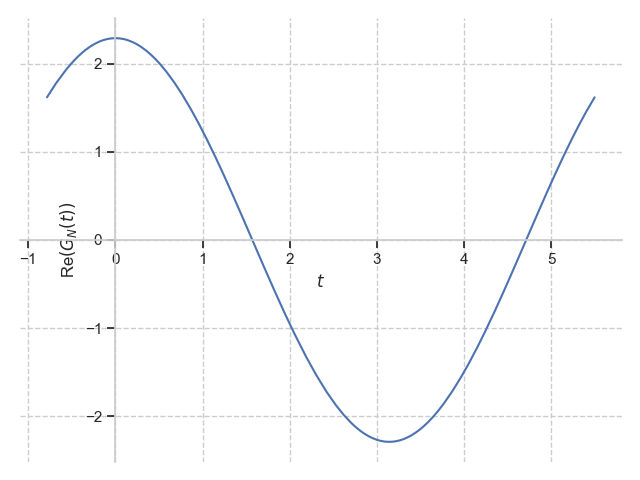
\includegraphics[scale=0.8]{fourier_re_cfunc_n=2.png}
    \captionsetup{skip=0pt}
    \caption{График Re$\,G_N(t)$ комплекснозначной функции при N=2}
    \label{Рис:44}
\end{figure}
\begin{figure}[!htb]
    \centering
    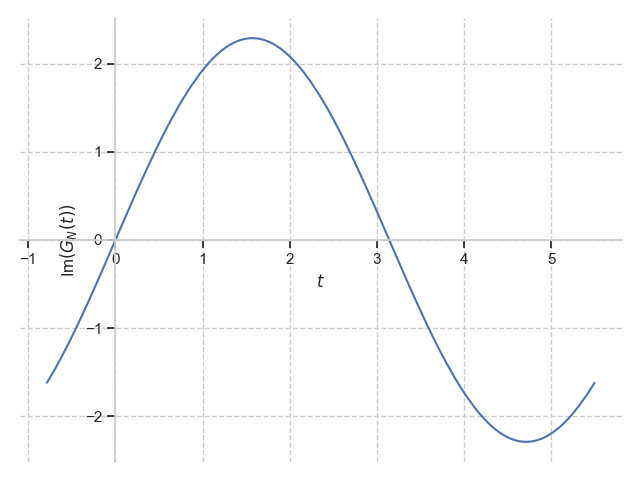
\includegraphics[scale=0.8]{fourier_im_cfunc_n=2.png}
    \captionsetup{skip=0pt}
    \caption{График Im$\,G_N(t)$ комплекснозначной функции при N=2}
    \label{Рис:45}
\end{figure}
\newpage
\vspace*{10mm}
\begin{figure}[!htb]
    \centering
    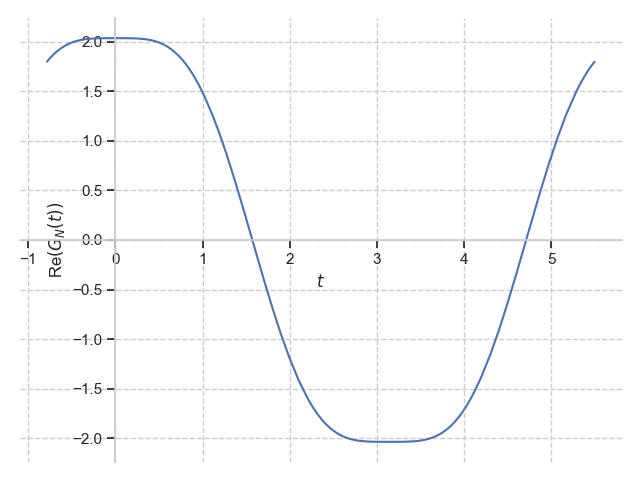
\includegraphics[scale=0.8]{fourier_re_cfunc_n=3.png}
    \captionsetup{skip=0pt}
    \caption{График Re$\,G_N(t)$ комплекснозначной функции при N=3}
    \label{Рис:46}
\end{figure}
\begin{figure}[!htb]
    \centering
    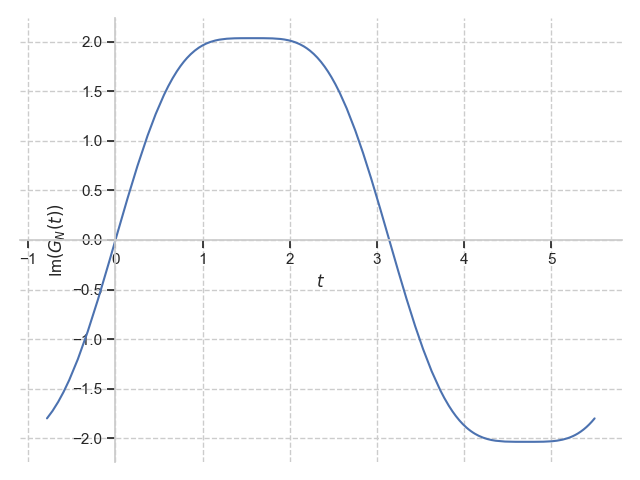
\includegraphics[scale=0.8]{fourier_im_cfunc_n=3.png}
    \captionsetup{skip=0pt}
    \caption{График Im$\,G_N(t)$ комплекснозначной функции при N=3}
    \label{Рис:47}
\end{figure}
\newpage
\begin{figure}[!htb]
    \centering
    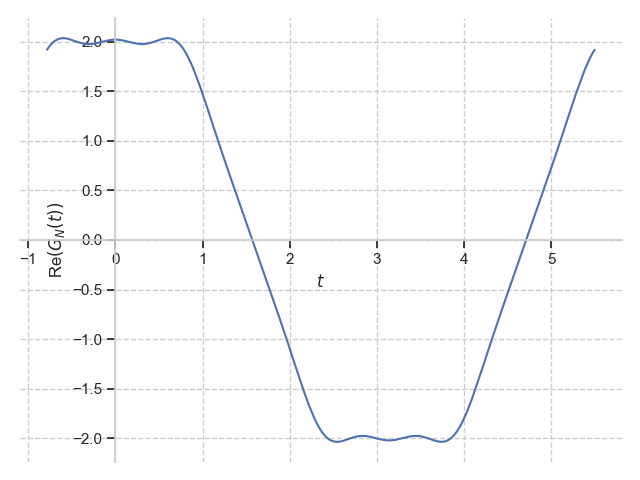
\includegraphics[scale=0.8]{fourier_re_cfunc_n=10.png}
    \captionsetup{skip=0pt}
    \caption{График Re$\,G_N(t)$ комплекснозначной функции при N=10}
    \label{Рис:48}
\end{figure}
\begin{figure}[!htb]
    \centering
    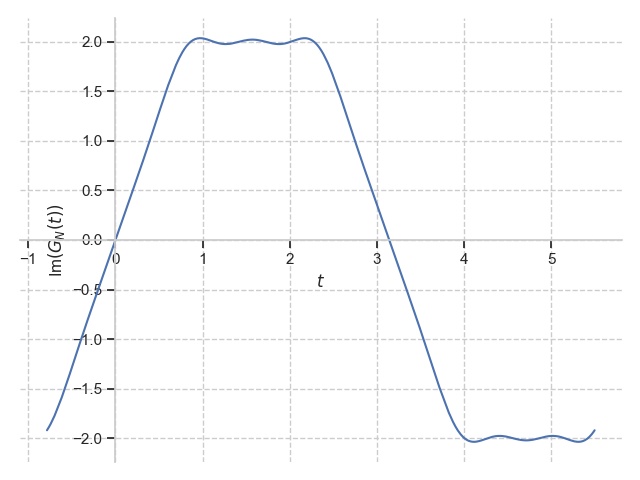
\includegraphics[scale=0.8]{fourier_im_cfunc_n=10.png}
    \captionsetup{skip=0pt}
    \caption{График Im$\,G_N(t)$ комплекснозначной функции при N=10}
    \label{Рис:49}
\end{figure}


\noindent Видим, как при увеличении N график Re$\,G_N(t)$ стремится к Re$\,f(t)$,
а Im$\,G_N(t)$ к Im$\,f(t)$. График функции Re$\,f(t)$ и графики функции Re$\,G_N(t)$ симметричны 
относительно оси ординат, что означает, что мы видим чётную функцию. Значит
график функции Re$\,G_N(t)$ так или иначе является графиком суммы косинусов. График функции Im$\,f(t)$
и графики функции Im$\,G_N(t)$ симметричны относительно начала координат, то есть представляют собой
нечётную функцию, значит так или иначе график функции Im$\,G_N(t)$ является графиком суммы синусов


\newpage
\noindent Проверим равенство Парсеваля тем же кодом, что и ранее. Результат при N=10:
\begin{lstlisting}
coeffs_sum=5.33247424348813    sqf_res=5.33333333333332
\end{lstlisting}


\noindent Результат при N=25:
\begin{lstlisting}
coeffs_sum=5.33328363761286    sqf_res=5.33333333333332
\end{lstlisting}


\noindent Результат при N=50:
\begin{lstlisting}
coeffs_sum=5.33332633068821    sqf_res=5.33333333333332
\end{lstlisting}


\noindent Результат при N=100:
\begin{lstlisting}
coeffs_sum=5.33333245747799    sqf_res=5.33333333333332
\end{lstlisting}


\noindent Видим, что сумма коэффициентов стремится к равенству Парсеваля, но в чистом
виде оно не выполняется


\section{Вывод}
\noindent В ходе выполнения работы я расширил свои знания о ряде Фурье, научился
строить графики ряда Фурье, проанализировал построенные графики,
познакомился с равенством Парсеваля и проверил его выполнение для каждой функции
\end{document}
